%% SpecBraM -- arXiv version (AAAI template, preprint mode: authors shown,
%% no AAAI copyright line; no page limit). Tables are generated by
%% make_arxiv_tables.py from results/arxiv_data -- do not edit tables/*.tex.
%% Build: pdflatex -> bibtex -> pdflatex -> pdflatex
\documentclass[letterpaper]{article}
\usepackage[preprint]{aaai2027}
\usepackage[hyphens]{url}
\usepackage{graphicx}
\urlstyle{rm}
\def\UrlFont{\rm}
\usepackage{natbib}
\usepackage{caption}
\frenchspacing
\usepackage{booktabs}
\usepackage{multirow}
\usepackage{amsmath,amssymb,amsthm,bm}
\usepackage{xcolor}
\usepackage{tikz}
\pdfinfo{/TemplateVersion (2027.1)}

\setcounter{secnumdepth}{2}   % arXiv version: numbered sections so Sec./App. refs resolve
\newcommand{\val}[2]{#1\,{\scriptsize$\pm$#2}}
\newcommand{\ci}[3]{#1\,{\scriptsize[#2,\,#3]}}
\newcommand{\E}{\mathbb{E}}
\newcommand{\Var}{\operatorname{Var}}
\newtheorem{assumption}{Assumption}
\newtheorem{lemma}{Lemma}
\newtheorem{proposition}{Proposition}
\theoremstyle{remark}
\newtheorem*{remark}{Remark}

\title{SpecBraM: Efficient EEG Foundation Model Pretraining\\
by Predicting Masked Band Power}
% ------------------------------------------------------------------
% TODO before posting: replace with the real author list and affiliations.
\author{Author One\textsuperscript{\rm 1}, Author Two\textsuperscript{\rm 1}}
\affiliations{\textsuperscript{\rm 1}Affiliation\\ email@example.com}
% ------------------------------------------------------------------

\begin{document}
\maketitle

\begin{figure*}[!t]\centering
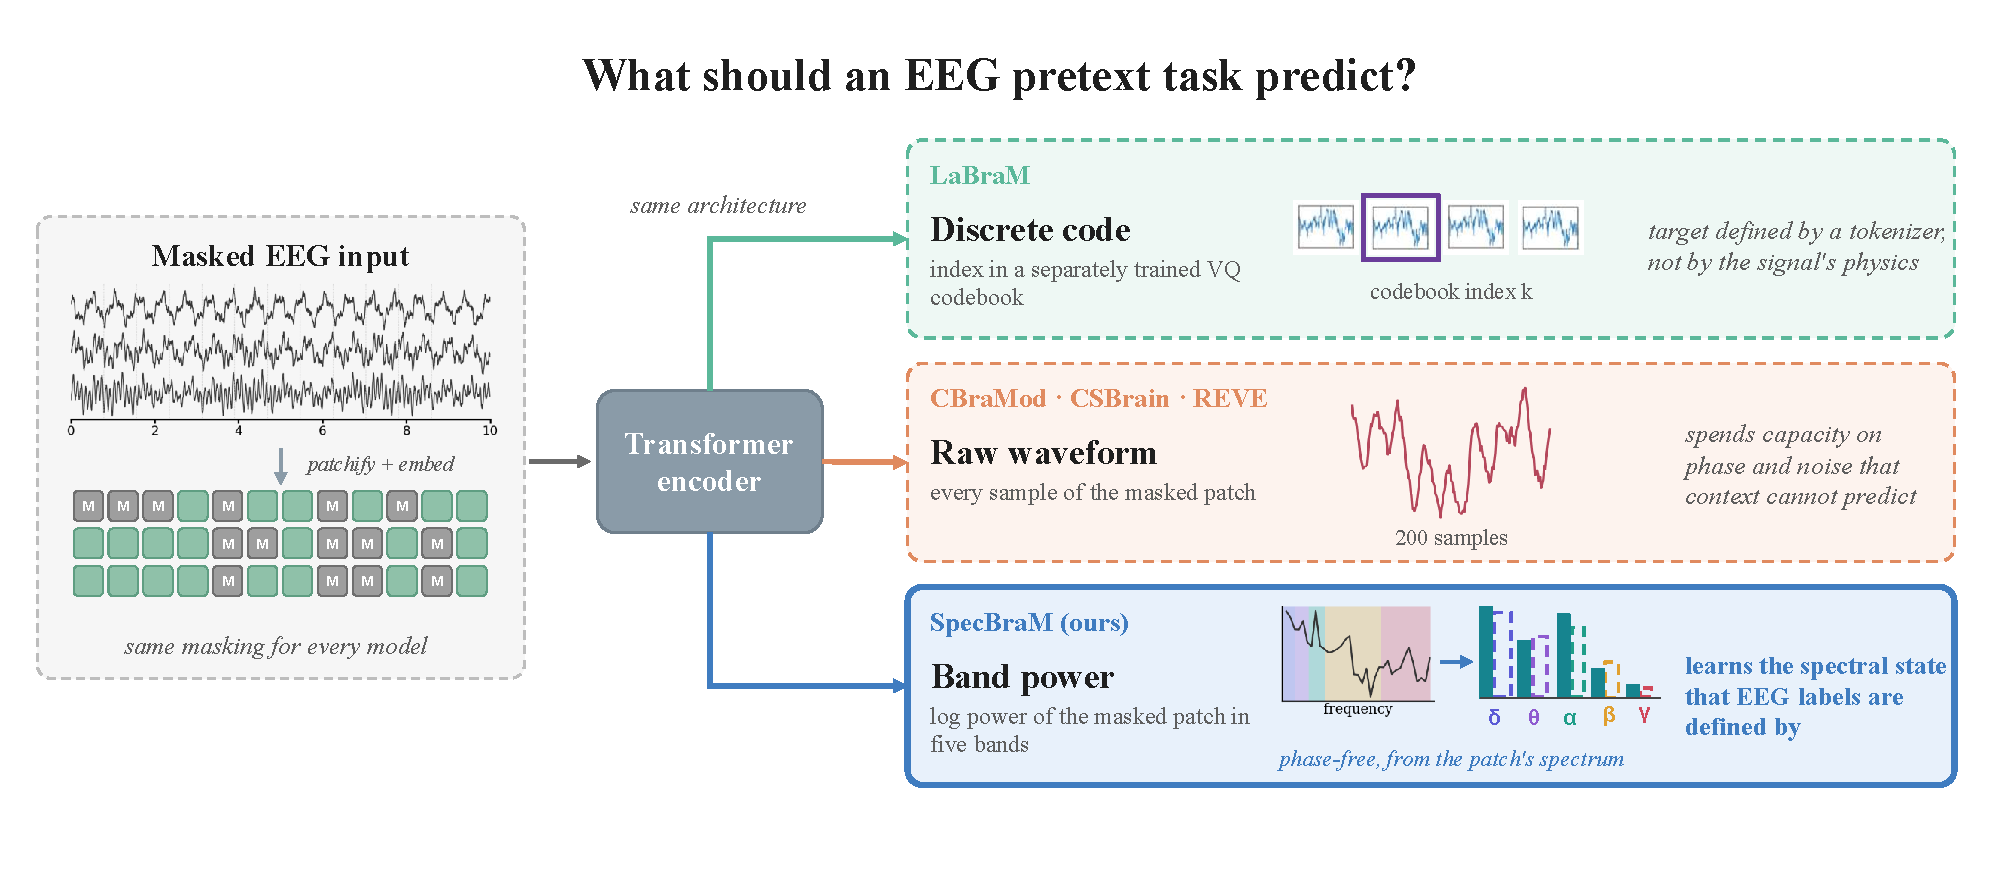
\includegraphics[width=0.98\textwidth]{figures/teaser.pdf}
\caption{\textbf{What should an EEG foundation model predict?} The model families encode the
same masked token grid with a transformer and differ in the pretraining target. LaBraM predicts
the discrete codes of a separately trained vector-quantized tokenizer; CBraMod, CSBrain and REVE
reconstruct every sample of the masked patch. SpecBraM predicts the log power of each masked
patch in the five classical frequency bands, computed from the patch's spectrum: a phase-invariant
physical quantity associated with the spectral state.}
\label{fig:contrast}
\end{figure*}

\begin{abstract}
EEG foundation models aim to decode brain states across clinical and cognitive tasks from few
labels. They are pretrained on large unlabeled corpora with objectives borrowed from images and
language, reconstructing the raw waveform of masked patches or predicting discrete tokens, and
their progress has come mainly from more data and larger models. These objectives also fit
waveform details beyond the spectral information relevant to many EEG labels. Sleep stages,
clinical slowing and many cognitive states are associated with the power of neural rhythms,
while a short patch also contains phase and sample-level variation that may be only partly
predictable from context. We present \textbf{SpecBraM}, an EEG foundation model pretrained by
\emph{masked band-power prediction}: from the visible context, it predicts the log power of each
masked (channel, time) patch in the classical frequency bands, a parameter-free physical target
computed from the patch's spectrum. Under an idealized spectral model, band-averaged power is
sufficient for the band levels, and its logarithm stabilizes sampling variance when the numerical
floor is ignored. This motivates a compact target for efficient learning. With backbone, data
and training steps fixed, the trained models explain substantially more of the band-power
target's variance than of the waveform's, and on sleep staging band-power pretraining reaches
the linear-probe quality of waveform reconstruction with a fraction of the steps and with a
model a tenth of the size. Under an identical strict linear probe on eight datasets spanning six task types,
SpecBraM, pretrained on a fraction of the data of recent models, outperforms CBraMod, LaBraM
and CSBrain on nearly all tasks and has higher point estimates than REVE, which uses far more
data, on most tasks. On sleep staging it also leads the compared models with few labelled
training epochs and in unsupervised clustering agreement.
\end{abstract}

% ======================================================================
\section{Introduction}
EEG is central to clinical neuroscience---sleep staging, screening for abnormal background
activity, studies of depression and cognitive load---but expert labels are scarce, which
motivates foundation models pretrained once on large unlabeled corpora such as the TUH EEG
Corpus (TUEG) \cite{obeid2016tuh} and transferred to many tasks
\cite{jiang2024labram,wang2025cbramod,csbrain,reve2025}. Their pretraining objectives are
borrowed from other modalities. LaBraM \cite{jiang2024labram} trains a vector-quantized
tokenizer and predicts its discrete codes, as BEiT does for images \cite{bao2022beit}; CBraMod
\cite{wang2025cbramod}, CSBrain \cite{csbrain} and REVE \cite{reve2025} reconstruct the raw
waveform of masked patches, as masked autoencoders reconstruct pixels \cite{he2022mae}. Progress
has come mainly from larger models and more data: REVE pretrains on about 60{,}000 hours.

We present \textbf{SpecBraM}, an EEG foundation model whose pretraining target is a physical
quantity rather than the signal. Spectral power informs many EEG labels: AASM sleep
stages are specified by the amount of delta activity, spindles and alpha
\cite{berry2017aasm}, clinical reports describe ``background slowing'', and quantitative EEG
uses band powers and their ratios. SpecBraM therefore keeps the standard masked-patch
transformer but, for each masked (channel, time) patch, predicts its log power in the five
classical frequency bands, computed from the patch's own spectrum (Fig.~\ref{fig:contrast}). The
target needs no tokenizer and no target network and costs one FFT per patch.

This target makes pretraining efficient, and we motivate a possible mechanism
(Sec.~\ref{sec:theory}). Under squared error, variation remaining after conditioning on the
visible context contributes gradient variance but no expected gradient. In an idealized
stationary-Gaussian Whittle model, marginal Fourier phases are ancillary for spectral
parameters; this does not imply that context cannot predict phase. With exactly flat bands
and observation restricted to those bands, the band-averaged periodogram is sufficient for
the band levels and is their maximum-likelihood estimate. Its zero-floor logarithm has
state-independent conditional sampling variance. These properties motivate a compact spectral
target, but do not prove lower gradient noise or faster optimization for the implemented model.

The experiments establish the efficiency gains. With backbone, data and steps fixed, band power reaches after one to two
pretraining epochs the linear-probe quality that waveform reconstruction reaches after sixteen,
and a band-power model with 4.2M parameters surpasses a waveform model with 51.3M. Pretrained on
2{,}388 hours, SpecBraM is evaluated with an identical strict linear probe on eight datasets
from six task types. Our contributions are:
\begin{itemize}
\item \textbf{SpecBraM}, an EEG foundation model pretrained by masked band-power prediction, a
parameter-free physical target that replaces waveform reconstruction (Sec.~\ref{sec:method}).
\item \textbf{An idealized rationale for the target}: band power summarizes state-associated
spectral levels without requiring phase prediction; risk and gradient decompositions clarify
the role of contextual uncertainty and target noise (Sec.~\ref{sec:theory},
Appendix~\ref{app:theory}).
\item \textbf{Evidence across tasks and in efficiency.} Under a strict linear probe SpecBraM
has higher point estimates than CBraMod, LaBraM and CSBrain on (nearly) all tasks and REVE on
most of them, using less pretraining data than several baselines. Matched target studies show
gains in pretraining steps, model size and low-label sleep probing
(Sec.~\ref{sec:results}).
\end{itemize}

\noindent We do not claim a new paradigm: masked prediction of hand-crafted features is
established in vision \cite{wei2022maskfeat} and speech \cite{hsu2021hubert}, and spectral
information enters the targets of several EEG models (Sec.~\ref{sec:related}).
This work was completed and submitted for peer review in July 2026; FAME
\cite{yu2026fame} and MANAS-2 \cite{kulkarni2026manas2}, which also use band log-power
targets, appeared afterwards and are concurrent.

% ======================================================================
\section{Related Work}\label{sec:related}
\noindent\textbf{EEG foundation models.} Early self-supervised EEG models used contrastive or
autoregressive objectives (BENDR \cite{kostas2021bendr}, Neuro-GPT \cite{cui2024neurogpt}).
Most recent models pretrain a transformer on TUEG with a masked-prediction objective: CBraMod
\cite{wang2025cbramod}, CSBrain \cite{csbrain} and REVE \cite{reve2025} reconstruct the raw
waveform of masked patches; LaBraM \cite{jiang2024labram} predicts the codes of a
vector-quantized tokenizer; EEGPT \cite{wang2024eegpt} combines reconstruction with latent
alignment; NeuroLM \cite{jiang2025neurolm} maps EEG to language tokens; BIOT
\cite{yang2023biot} handles heterogeneous biosignals. These models differ mainly in
architecture, scale and data, while their targets are inherited from vision and language. A
waveform target asks the model to predict sample-level details, including phase, in addition
to spectral structure; some of this variation may remain uncertain given the context. A
learned codebook target is defined by a tokenizer rather than by a physiological quantity. Our
target directly measures band power, a spectral quantity relevant to many EEG labels.

\noindent\textbf{Spectral information in EEG pretraining.} Spectral features enter several
models as inputs or tokenizers: BIOT tokenizes STFT magnitudes, CBraMod adds a
frequency-domain patch embedding, LaBraM's tokenizer reconstructs the Fourier amplitude and
phase, BioSerenity-E1 \cite{bettinardi2025bioserenity} and BandVQ \cite{sukhbaatar2026bandvq}
quantize log spectra, and BrainBERT \cite{wang2023brainbert} reconstructs intracranial
spectrograms. Concurrently, FAME \cite{yu2026fame} decodes band-averaged log power of the whole
sequence to counter the low-frequency bias of masked autoencoders, and MANAS-2
\cite{kulkarni2026manas2} adds band log-power to waveform reconstruction. In these works
spectral information is an input, a quantized code or an auxiliary term, and its role as the
target is neither motivated nor isolated. We use band power of the masked patches as the sole
target, derive it from a likelihood argument, and isolate its effect with matched controls.

\noindent\textbf{Feature and latent prediction.} In vision and speech, predicting fixed
hand-crafted features of masked inputs (HOG in MaskFeat \cite{wei2022maskfeat}, MFCC clusters in
HuBERT \cite{hsu2021hubert}) can outperform predicting the raw signal, and latent-predictive
methods (I-JEPA \cite{assran2023ijepa}, data2vec \cite{baevski2022data2vec}, EEG2Rep
\cite{foumani2024eeg2rep}) predict learned representations but need anti-collapse mechanisms
such as SIGReg \cite{balestriero2025lejepa}. Band power plays the role of such a feature for
EEG: it is a physiological quantity relevant to many labels, and we use the fixed target
without an explicit anti-collapse regularizer.

% ======================================================================
\section{SpecBraM}\label{sec:method}
\begin{figure*}[t]\centering
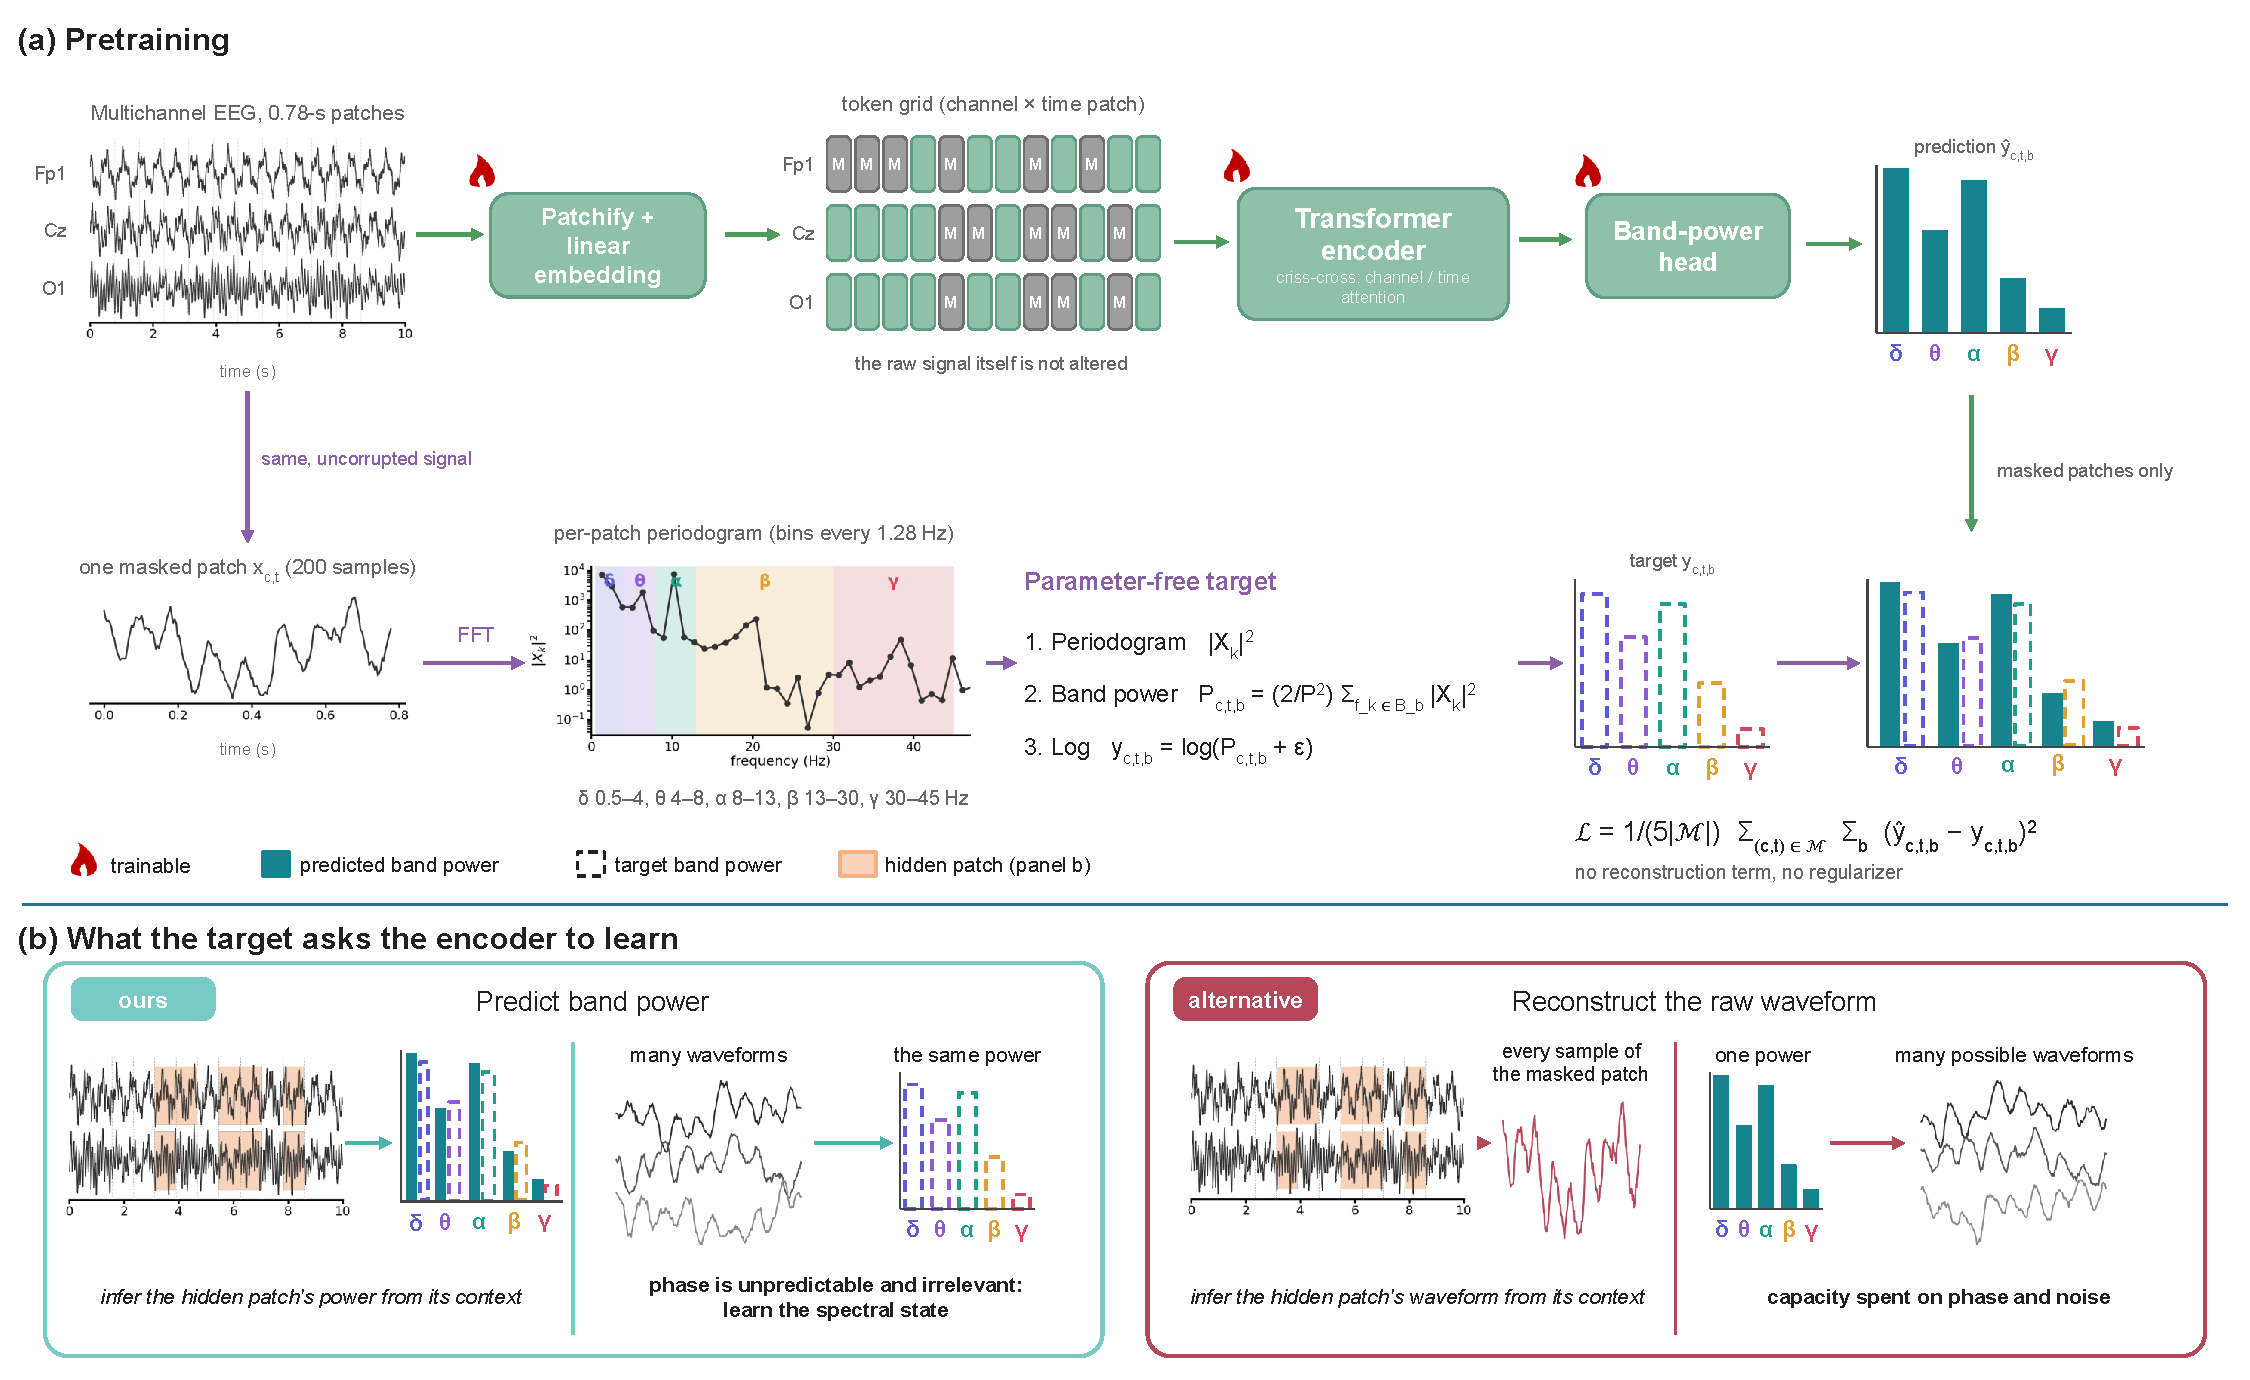
\includegraphics[width=\textwidth]{figures/pipeline_v2.pdf}
\caption{\textbf{SpecBraM pretraining.} (a) Each channel is cut into 0.78-s patches that are
embedded linearly; 30\% of the (channel, time) tokens are replaced by a learnable [M] token,
while the signal itself is not altered. A criss-cross transformer encodes the token grid and a
linear head predicts five log band powers for every masked token. The target is computed from
the periodogram of the uncorrupted patch and has no parameters. (b) Predicting band power asks
the encoder to infer the spectral state of a hidden patch from its context; reconstructing the
waveform also asks for sample-level details, including phase, that the context may only
partly determine.}
\label{fig:pipeline}
\end{figure*}
\noindent\textbf{Input and tokens.} A 10-s window at 256\,Hz over the 19 channels of the
10--20 montage, normalized per recording (median and interquartile range), is cut per channel
into non-overlapping patches of $P{=}200$ samples ($0.78$\,s), giving a token grid with
$C{=}19$ channels and $T_p{=}\lfloor 2560/200\rfloor{=}12$ time patches; the last 160 samples
($0.625$\,s) of each window are not used, during pretraining and in every downstream window
(including each of the three 10-s windows of a 30-s sleep epoch; 5-s TUEV windows give six
patches). The main model embeds each patch with a single
linear map (as CBraMod does). A variant decomposes each patch with a learnable 5-band
filterbank before embedding (``filterbank tokenizer''); we report both because the target
study crosses tokenizer and target.

\noindent\textbf{Encoder and masking.} A 12-layer criss-cross transformer ($D{=}512$, 8 heads;
51.3M parameters) alternates attention along the channel and time axes, with learned channel
and time position embeddings. Each (channel, time) patch is masked independently with
probability $0.3$; the embeddings of masked patches are replaced by a learned mask token.

\noindent\textbf{Target.} For each patch $\bm{x}_{c,t}\in\mathbb{R}^{P}$ of the uncorrupted
signal, let $X_k=\sum_{\tau}x_{c,t,\tau}e^{-i2\pi k\tau/P}$ be its discrete Fourier transform
(rectangular window, no padding) at $f_k=kf_s/P$. For the five classical bands
$B_1,\dots,B_5=[0.5,4),[4,8),[8,13),[13,30),[30,45)$\,Hz
($\delta,\theta,\alpha,\beta,\gamma$),
\begin{align}
P_{c,t,b}&=\frac{2}{P^2}\sum_{f_k\in B_b}|X_k|^2,\nonumber\\
y_{c,t,b}&=\log\bigl(P_{c,t,b}+\varepsilon\bigr),\qquad b=1,\dots,5, \label{eq:target}
\end{align}
with $\varepsilon=10^{-3}$ in the robust-scaled input units; its effect depends on the band
power relative to this floor. By one-sided Parseval, $P_{c,t,b}$ is the variance of
the patch within band $b$; it equals the band-averaged periodogram of Sec.~\ref{sec:theory}
times the per-band constant $2m_b/P$, where $m_b$ is the number of Fourier bins in the band
(3/3/4/13/12 at $\Delta f=1.28$\,Hz; Table~\ref{tab:bins}). The target is fixed (no learnable
parameters) and patch-local: it uses no samples of neighbouring, possibly visible patches.

\noindent\textbf{Choice of bands.} The classical partition reflects physiologically distinct
rhythms (slow-wave activity, theta, the posterior alpha rhythm and sleep spindles at its upper
edge, beta and gamma) and is the vocabulary in which sleep scoring and clinical EEG reports are
written. Its exact edges are conventions (alpha is given as 8--12 or 8--13\,Hz, and individual
alpha frequency varies by several hertz), so we treat them as a sensible default rather than
an optimum.

\noindent\textbf{Objective.} A linear head maps each encoder output $H_{c,t}$ to five
predictions $\hat y_{c,t,b}$. With $\mathcal{M}$ the set of masked patches,
\begin{equation}
\mathcal{L}=\frac{1}{5|\mathcal{M}|}\sum_{(c,t)\in\mathcal{M}}\sum_{b=1}^{5}
\bigl(\hat y_{c,t,b}-y_{c,t,b}\bigr)^2,
\label{eq:loss}
\end{equation}
the mean squared error over the masked patches and the five bands. There is no
reconstruction term, no latent-prediction term and no regularizer. The target is fixed;
this alone does not guarantee a noncollapsed representation. The waveform-reconstruction controls replace the loss of
Eq.~\eqref{eq:loss} by the MSE between a linear decoder output and the raw samples of each
masked patch (``raw'') or five band-pass-filtered versions of the patch waveform (fixed 65-tap
Hann-windowed cosine filters centred at 2/6/10/21/38\,Hz; ``band-waveform''), with everything
else unchanged.

% ======================================================================
\section{Why Predicting Band Power Is Efficient}\label{sec:theory}
We motivate the target under an idealized model; the statements and proofs are in
Appendix~\ref{app:theory}. Before the logarithm and numerical floor, the main target,
Eq.~\eqref{eq:target}, is a per-band constant times the band-averaged periodogram. The exact
log-noise identities below apply to the zero-floor idealization with independent Fourier bins
and exactly flat in-band spectra. The implemented $\log(P+\varepsilon)$ and real EEG need not
satisfy them. The analysis motivates the target and suggests empirical hypotheses; it is not a
proof of optimality or an optimization-speed guarantee.

\noindent\emph{Model.} Given a brain state $\theta$, a patch is a segment of a zero-mean
stationary Gaussian process with spectral density $S_\theta$; the state acts on the data only
through $S_\theta$. Asymptotically, the discrete Fourier coefficients at distinct frequencies
are independent circular complex Gaussians, so the periodogram ordinates are $I_k\approx
S_\theta(f_k)E_k$ with $E_k\sim\mathrm{Exp}(1)$, and the phases are uniform and independent of
$\theta$ \cite{brillinger1981}. The Whittle likelihood \cite{whittle1953} depends on the data
only through $\{I_k\}$.

\noindent\emph{What band power keeps.} (i) In the Whittle model, the periodogram is sufficient
for its spectral parameters and the marginal phases are ancillary (Prop.~\ref{prop:suff});
this does not establish independence from visible context. (ii) With exactly constant in-band
spectra and observation restricted to those bins, the band-averaged periodogram is sufficient
for the band levels and is their maximum-likelihood estimate (Prop.~\ref{prop:mle}). (iii)
For its zero-floor logarithm, $\Var[\log P_b\mid\theta]=\psi'(m_b)\approx 1/m_b$ is independent
of the state (Prop.~\ref{prop:var}). This motivates variance stabilization, but neither
sufficiency for arbitrary EEG labels nor an exact noise model for Eq.~\eqref{eq:target} follows.

\noindent\emph{A possible learning advantage.} Under squared error, prediction risk splits
into error relative to $g(\bm{c})=\E[Y\mid\bm{c}]$ and the Bayes risk given the fixed context
(Prop.~\ref{prop:decomp}). Only the former can be reduced by improving the predictor.
Under an additional independent-patch idealization, the zero-floor band-power predictor is
$\E[\log s_b(\theta)\mid\bm{c}]+\text{const}$, a posterior average of spectral levels,
rather than the state itself. Its conditional variance contains both $\psi'(m_b)$ and posterior
uncertainty about $\log s_b(\theta)$. In this same independence model the zero-mean waveform
predictor would be zero. A separate correlated Gaussian model instead yields Wiener
interpolation conditional on the state, with additional uncertainty when the state is unknown.
For either target, the full conditional covariance contributes Jacobian-weighted gradient
noise (Prop.~\ref{prop:grad}). Standard SGD upper bounds can worsen with gradient variance
\cite{ghadimi2013}, but the two targets also differ in conditional mean, dimension, scale and
Jacobian. These identities suggest a possible advantage of a compact spectral target; they do
not establish an ordering of gradient noise or steps to a given downstream score.

\noindent\emph{Predictions.} (P1) At matched backbone, data and steps, band power should give
representations that are easier to read out linearly, especially with few labels. (P2) It should
reach a given quality with fewer pretraining steps and smaller models. (P3) Reconstructing
band-filtered \emph{waveforms} need not yield the same gains, since they still require sample-level prediction.
(P4) The advantage should shrink for tasks that depend on transient waveform shape or
cross-channel phase relations. Sec.~\ref{sec:results} tests these.

% ======================================================================
\section{Experimental Setup}\label{sec:setup}
\noindent\textbf{Pretraining.} TUEG v2.0.1 at 256\,Hz, 10-s windows, per-recording robust
normalization, with recordings shorter than 5\,min dropped, 60\,s trimmed from each end and
windows exceeding $150\,\mu$V rejected. All models use a random subset of 2{,}100 patients
(859{,}606 windows, 2{,}388\,h; the same subset for every run), AdamW (learning rate
$1.7{\times}10^{-3}$, weight decay $0.05$), 7 warm-up epochs and a cosine schedule defined
over 105 epochs, stopped after epoch 16 for every run (matched steps), effective batch 512 on
four RTX A6000 GPUs. Pretraining seeds 42/43/44 change initialization and data order on the
same subset. Downstream patients are not excluded from pretraining (as in prior work).

\noindent\textbf{Strict linear probe (primary metric)}\label{sec:lpproto}. The encoder is
frozen; the tokens of a window are mean-pooled; features are standardized on the training
split; a class-balanced logistic regression is fitted with $C\in\{0.01,0.1,1\}$ selected on the
validation split by balanced accuracy, and the test split is scored once. For sleep, a 30-s
epoch is the mean of its three 10-s window features. The probe is deterministic, so baselines
with a single released checkpoint need no repetitions; our models are reported over three
pretraining seeds. Sleep label efficiency reuses the full-label-selected $C$ on 1--50\% of the
training epochs (five fixed random subsets, identical for all models); these fractions do not
include the labels used for hyperparameter selection and do not subsample subjects. Each model receives the same
samples in its own documented input convention: ours at 256\,Hz with per-recording robust
scaling on the 19 standard leads; CBraMod and LaBraM at 200\,Hz, raw $\mu$V$/100$, with the
recording's own channels (LaBraM by its channel names); BIOT with its 95th-percentile scaling
on C3/C4 fed to its C3--A2/C4--A1 channel tokens; CSBrain as CBraMod, with the brain-region
layout of its own wrapper for each dataset; REVE at 200\,Hz with per-recording z-scoring clipped
at ${\pm}15$ SD and its own electrode-position bank. We compare with released models of
comparable size (3--70M parameters: BIOT, CBraMod, LaBraM-Base, CSBrain, REVE-Base; ours 51M);
REVE-Large (390M) belongs to a different scale class and is not included. Every baseline is
measured with this probe; no linear-probe number is quoted from other papers. For REVE, the readout (mean pooling, or its own pretrained attention pooling; both
frozen and fitted without downstream labels) is selected using validation labels, like $C$.

\noindent\textbf{Downstream tasks.} We evaluate on eight public datasets from six task types:
sleep staging (ISRUC \cite{khalighi2016isruc}, HMC \cite{alvarez2021hmc}; five stages),
clinical EEG (abnormality detection on TUAB and six-class event classification on TUEV
\cite{obeid2016tuh}), mental workload (MA \cite{zyma2019mentalarith}), depression (Mumtaz
\cite{mumtaz2016mdd}), emotion recognition (FACED \cite{chen2023faced}, nine classes) and motor
imagery (PhysioNet-MI \cite{schalk2004bci2000}, four classes). We reproduce the preprocessing
and split protocols of CBraMod and CSBrain, with matching sample counts. In TUAB's original
per-class training/validation split, three patients occur in both splits; its test patients are
disjoint from both. This limits validation independence and is separate from possible TUEG
pretraining overlap. TUEV has no patient overlap among its downstream splits.
Appendix~\ref{app:fullmetrics} describes every dataset.

% ======================================================================
\section{Results}\label{sec:results}

% auto-generated by make_arxiv_tables.py -- do not edit
\begin{table*}[t]\centering\small
\setlength{\tabcolsep}{3.5pt}
\caption{\textbf{Strict linear probe across task types} (balanced accuracy). Frozen encoder,
mean-pooled tokens, logistic regression with $C$ selected on the validation split, test scored
once; every model sees the identical samples and splits in its own input convention
(Sec.~\ref{sec:lpproto}), and every number is measured by us with the publicly released
weights. Every model is one checkpoint: SpecBraM is our main released checkpoint, the
baselines are their released ones. Brackets: 95\% confidence interval from 1{,}000 bootstrap
resamples of the test subjects (TUEV: recordings); the spread over our three pretraining seeds
is given in Appendix~\ref{app:fullmetrics}. REVE: readout selected on the validation split. BIOT's
released channel tokens cover only the sleep montage. Per-dataset results with Cohen's $\kappa$,
weighted F1 and AUROC/AUC-PR: Appendix~\ref{app:fullmetrics}. Bold: best per column.}
\label{tab:overview}
\resizebox{\textwidth}{!}{%
\begin{tabular}{l c cc cc c c c c}
\toprule
& & \multicolumn{2}{c}{Sleep staging} & \multicolumn{2}{c}{Clinical EEG} & \multicolumn{1}{c}{Workload} & \multicolumn{1}{c}{Depression} & \multicolumn{1}{c}{Emotion} & \multicolumn{1}{c}{Motor imagery}\\
\cmidrule(lr){3-4}\cmidrule(lr){5-6}\cmidrule(lr){7-7}\cmidrule(lr){8-8}\cmidrule(lr){9-9}\cmidrule(lr){10-10}
Model & Pretraining & ISRUC & HMC & TUAB & TUEV & MA & Mumtaz & FACED & PhysioNet-MI\\
\midrule
\textbf{SpecBraM} & $2{,}388$\,h & \ci{0.790}{0.764}{0.816} & \ci{\textbf{0.742}}{0.699}{0.776} & \ci{0.813}{0.775}{0.850} & \ci{0.555}{0.491}{0.648} & \ci{\textbf{0.781}}{0.722}{0.840} & \ci{\textbf{0.939}}{0.868}{0.995} & \ci{\textbf{0.221}}{0.195}{0.248} & \ci{\textbf{0.417}}{0.384}{0.450} \\
CBraMod & ${\sim}9$k\,h & \ci{0.728}{0.702}{0.752} & \ci{0.619}{0.576}{0.654} & \ci{0.778}{0.738}{0.814} & \ci{0.525}{0.471}{0.609} & \ci{0.653}{0.507}{0.799} & \ci{0.893}{0.760}{0.988} & \ci{0.171}{0.156}{0.188} & \ci{0.312}{0.286}{0.340} \\
LaBraM-Base & ${\sim}2.5$k\,h & \ci{0.752}{0.720}{0.777} & \ci{0.632}{0.583}{0.673} & \ci{0.776}{0.740}{0.812} & \ci{0.468}{0.416}{0.545} & \ci{0.681}{0.597}{0.736} & \ci{0.876}{0.744}{0.986} & \ci{0.167}{0.152}{0.181} & \ci{0.299}{0.285}{0.314} \\
BIOT & mixed & \ci{0.736}{0.691}{0.771} & \ci{0.658}{0.609}{0.697} & -- & -- & -- & -- & -- & -- \\
CSBrain & ${\sim}9$k\,h & \ci{0.730}{0.706}{0.752} & \ci{0.611}{0.580}{0.641} & \ci{0.772}{0.736}{0.805} & \ci{\textbf{0.564}}{0.505}{0.621} & \ci{0.556}{0.403}{0.653} & \ci{0.864}{0.774}{0.943} & \ci{0.179}{0.161}{0.199} & \ci{0.298}{0.273}{0.325} \\
REVE-Base & ${\sim}60$k\,h & \ci{\textbf{0.793}}{0.765}{0.816} & \ci{0.704}{0.664}{0.737} & \ci{\textbf{0.821}}{0.781}{0.861} & \ci{0.546}{0.500}{0.587} & \ci{0.684}{0.562}{0.771} & \ci{0.902}{0.743}{0.994} & \ci{0.200}{0.179}{0.225} & \ci{0.403}{0.371}{0.438} \\
\bottomrule
\end{tabular}}
\end{table*}


\subsection{Strict linear probe across tasks}\label{sec:lpfm}
Table~\ref{tab:overview} summarizes the strict linear probe on all tasks, grouped by task type.
As for the external models, which are released as single checkpoints, we evaluate one
checkpoint of SpecBraM, our main released model, and give every model a 95\% confidence
interval from 1{,}000 bootstrap resamples of the test subjects (TUEV: recordings). SpecBraM has
higher point estimates than CBraMod and LaBraM on every task, BIOT on sleep staging, and CSBrain
on every task except event classification (TUEV $0.555$ vs.\ $0.564$). REVE, of similar size but
pretrained on about 25 times more data, is the strongest baseline. On \emph{sleep staging}
SpecBraM has no detected difference on ISRUC ($0.790$ vs.\ $0.793$) and a higher point estimate on HMC ($0.742$ vs.\
$0.704$); on \emph{workload}, \emph{depression}, \emph{emotion} and \emph{motor imagery} its
point estimates are higher (mental arithmetic $0.781$ vs.\ $0.684$, Mumtaz $0.939$ vs.\ $0.902$, FACED $0.221$ vs.\
$0.200$, PhysioNet-MI $0.417$ vs.\ $0.403$); on \emph{clinical EEG} there is no detected
difference on event classification (TUEV $0.555$ vs.\ $0.546$), and its abnormality-detection point estimate is lower (TUAB $0.813$
vs.\ $0.821$). The intervals are wide for the small cohorts (mental arithmetic has four test
subjects, Mumtaz eleven), and the TUH tasks share corpus provenance with TUEG; their patients
were not excluded from our pretraining. Table~\ref{tab:paired} reports nominal, unadjusted
paired bootstrap intervals for the differences (Appendix~\ref{app:fullmetrics}). Intervals
containing zero indicate no detected difference under this procedure, not equivalence.
Appendix~\ref{app:fullmetrics} reports Cohen's $\kappa$, weighted F1 and, for
binary tasks, AUROC and AUC-PR for every dataset, together with the mean and standard deviation
over our three pretraining seeds.

Model size, input convention and readout also differ between the models; varying each in turn
(Appendix~\ref{app:confounds}) does not close the gap to CBraMod and LaBraM. Although our focus
is frozen use, SpecBraM also fine-tunes well: with full fine-tuning on sleep staging it reaches
$0.818$/$0.770$ balanced accuracy on ISRUC/HMC, above the listed published point estimates of
CBraMod, CSBrain and REVE under their respective recipes (Appendix~\ref{app:fttasks}).

\IfFileExists{tables/compute.tex}{% auto-generated by make_arxiv_tables.py -- do not edit
\begin{table}[t]\centering\small
\caption{\textbf{Along pretraining} (linear patch embedding, seed 42, strict linear probe BA;
bold: better target at that epoch).}
\label{tab:compute}
\begin{tabular}{c cc cc}
\toprule
& \multicolumn{2}{c}{ISRUC} & \multicolumn{2}{c}{HMC}\\
\cmidrule(lr){2-3}\cmidrule(lr){4-5}
Epoch & BP & Raw & BP & Raw\\
\midrule
1 & \textbf{0.7716} & 0.7398 & \textbf{0.7125} & 0.6593 \\
2 & \textbf{0.7812} & 0.7411 & \textbf{0.7222} & 0.6664 \\
4 & \textbf{0.7866} & 0.7431 & \textbf{0.7276} & 0.6689 \\
8 & \textbf{0.7904} & 0.7572 & \textbf{0.7477} & 0.7140 \\
12 & \textbf{0.7904} & 0.7688 & \textbf{0.7364} & 0.7160 \\
16 & \textbf{0.7901} & 0.7627 & \textbf{0.7420} & 0.7152 \\
\bottomrule
\end{tabular}
\end{table}
}{}
\IfFileExists{tables/target_r2.tex}{% auto-generated by make_arxiv_tables.py -- do not edit
\begin{table}[t]\centering\small
\caption{\textbf{How much of its pretraining target each model predicts}: fraction of the
target variance explained, $R^2=1-\mathrm{MSE}/\mathrm{Var}$, on the masked patches of 4{,}000
held-out windows (TUAB evaluation split, not excluded from TUEG pretraining; masks as in
pretraining), along pretraining (seed 42) and at the end over three seeds.
BP: mean of the five per-band $R^2$ values; waveform: pooled-sample $R^2$.
These are achieved scores, not estimates of Bayes ceilings. Band power, per band
$\delta/\theta/\alpha/\beta/\gamma$ at epoch 16: 0.89 / 0.89 / 0.92 / 0.94 / 0.95.}
\label{tab:target_r2}
\setlength{\tabcolsep}{6pt}
\begin{tabular}{l cc}
\toprule
Epoch & Band power & Raw waveform\\
\midrule
1 & 0.801 & 0.012 \\
2 & 0.880 & 0.016 \\
4 & 0.902 & 0.021 \\
8 & 0.909 & 0.025 \\
12 & 0.916 & 0.028 \\
16 & 0.917 & 0.031 \\
\midrule
16, three seeds & \val{0.917}{0.001} & \val{0.030}{0.000} \\
\bottomrule
\end{tabular}
\end{table}
}{}
% auto-generated by make_arxiv_tables.py -- do not edit
\begin{table}[t]\centering\small
\setlength{\tabcolsep}{3pt}
\caption{\textbf{Label efficiency} (strict linear probe, balanced accuracy vs.\ fraction of
labelled training epochs; ${<}100\%$: mean of five fixed random subsets shared by all
models). SpecBraM: main checkpoint. Bold: best per column.}
\label{tab:labeleff}
\resizebox{\columnwidth}{!}{%
\begin{tabular}{l cccccc}
\toprule
Model & 1\% & 5\% & 10\% & 25\% & 50\% & 100\%\\
\midrule
\multicolumn{7}{l}{\emph{ISRUC}}\\
BIOT & 0.655 & 0.703 & 0.716 & 0.728 & 0.734 & 0.736 \\
CBraMod & 0.660 & 0.709 & 0.717 & 0.726 & 0.727 & 0.729 \\
LaBraM-Base & 0.680 & 0.724 & 0.730 & 0.741 & 0.746 & 0.752 \\
CSBrain & 0.633 & 0.693 & 0.708 & 0.721 & 0.726 & 0.730 \\
REVE-Base & 0.736 & 0.771 & 0.778 & 0.788 & \textbf{0.791} & \textbf{0.792} \\
\textbf{SpecBraM} & \textbf{0.760} & \textbf{0.779} & \textbf{0.788} & \textbf{0.791} & \textbf{0.791} & 0.790 \\
\multicolumn{7}{l}{\emph{HMC}}\\
BIOT & 0.582 & 0.625 & 0.638 & 0.648 & 0.655 & 0.658 \\
CBraMod & 0.539 & 0.590 & 0.602 & 0.613 & 0.616 & 0.620 \\
LaBraM-Base & 0.574 & 0.616 & 0.621 & 0.630 & 0.631 & 0.633 \\
CSBrain & 0.509 & 0.581 & 0.595 & 0.608 & 0.612 & 0.612 \\
REVE-Base & 0.635 & 0.679 & 0.691 & 0.700 & 0.702 & 0.704 \\
\textbf{SpecBraM} & \textbf{0.662} & \textbf{0.698} & \textbf{0.717} & \textbf{0.733} & \textbf{0.738} & \textbf{0.742} \\
\bottomrule
\end{tabular}}
\end{table}


\begin{figure}[t]\centering
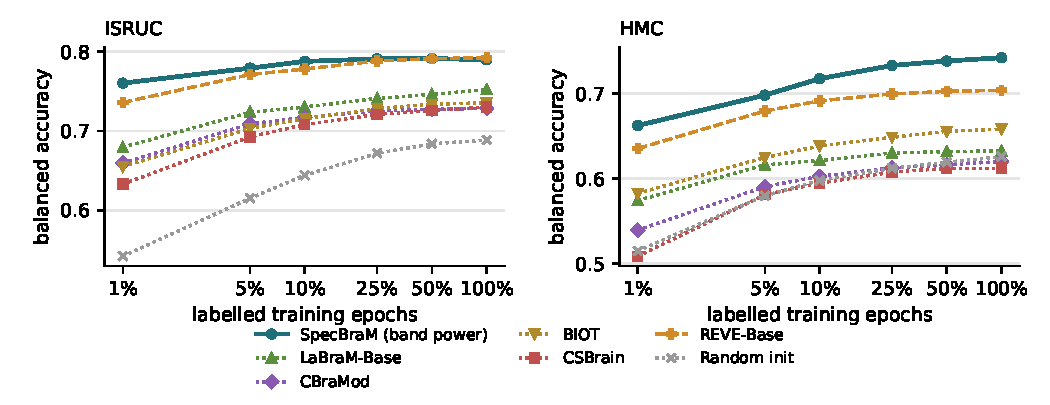
\includegraphics[width=\columnwidth]{figures/label_efficiency_lp.pdf}
\caption{\textbf{Label efficiency} under the strict linear probe (balanced accuracy;
SpecBraM: main checkpoint).}
\label{fig:labeleff}
\end{figure}

% auto-generated by make_arxiv_tables.py -- do not edit
\begin{table}[t]\centering\small
\setlength{\tabcolsep}{3.5pt}
\caption{\textbf{Clustering evaluation}: k-means ($k{=}5$) on frozen sleep features of the
test split (standardized, 64 PCA dimensions; cluster fitting uses no labels), agreement with the
expert stages. Mean over five k-means seeds; our rows: seed-42 checkpoints.
REVE: readout selected by validation NMI using labels. Bold: best per column.}
\label{tab:cluster}
\resizebox{\columnwidth}{!}{%
\begin{tabular}{l cc cc}
\toprule
& \multicolumn{2}{c}{ISRUC} & \multicolumn{2}{c}{HMC}\\
\cmidrule(lr){2-3}\cmidrule(lr){4-5}
Model & NMI & ARI & NMI & ARI\\
\midrule
\textbf{SpecBraM} & \textbf{0.417} & \textbf{0.310} & \textbf{0.236} & \textbf{0.179} \\
Raw-waveform recon.\ (same arch.) & 0.401 & 0.278 & 0.182 & 0.135 \\
\midrule
CBraMod & 0.277 & 0.184 & 0.083 & 0.056 \\
LaBraM-Base & 0.356 & 0.291 & 0.083 & 0.051 \\
BIOT & 0.149 & 0.091 & 0.057 & 0.025 \\
CSBrain & 0.263 & 0.166 & 0.069 & 0.038 \\
REVE-Base & 0.323 & 0.279 & 0.155 & 0.103 \\
\bottomrule
\end{tabular}}
\end{table}


\subsection{Efficiency}\label{sec:efficiency}
\noindent\textbf{Pretraining steps.} Table~\ref{tab:compute} follows the linear probe along
pretraining for the two targets, with everything else fixed. After a single epoch, band power
reaches $0.772$ on ISRUC, above raw-waveform reconstruction after sixteen epochs ($0.763$); on
HMC it is close after one epoch ($0.713$ vs.\ $0.715$) and exceeds it after two ($0.722$).
Band power thus reaches the final quality of waveform reconstruction with 8 to 16 times fewer
pretraining steps (P2). Target computation uses one FFT per
patch, the head has five outputs per patch instead of 200, no tokenizer is trained beforehand
(as for LaBraM) and no target network is maintained (as for latent prediction).

\noindent\textbf{Achieved target prediction.} Table~\ref{tab:target_r2} measures prediction
on TUAB evaluation windows with the masks of pretraining. These windows are held out from
downstream training; exclusion from pretraining is not established. The
band-power model explains $80\%$ of its target's variance after one epoch and $92\%$ after
sixteen; the waveform model explains $1.2\%$ after one epoch and $3.1\%$ after sixteen. Band-power
$R^2$ is averaged over the five per-band scores, whereas waveform $R^2$ pools the sample
coordinates. These are achieved scores, not Bayes predictability ceilings: residual error
combines contextual uncertainty with model and optimization error, and does not determine a
fraction of gradient noise. The early improvement of band-power prediction accompanies the
early rise of its linear probe.

\noindent\textbf{Model size and data.} At 4.2M parameters, the size of CBraMod, the band-power
model ($0.788$/$0.728$ on ISRUC/HMC) surpasses the 51.3M-parameter waveform model
($0.770$/$0.715$; Table~\ref{tab:ablation}), and it exceeds CBraMod, pretrained on about four
times more data, by $6.0$/$10.9$ points. SpecBraM is pretrained on $2{,}388$ hours, about a
quarter of the data of CBraMod and CSBrain and a twenty-fifth of REVE's, and ranks first on
most tasks of Table~\ref{tab:overview}.

\noindent\textbf{Labels.} On sleep staging, SpecBraM remains effective with few labelled
training epochs (Table~\ref{tab:labeleff}, Fig.~\ref{fig:labeleff}). With $1\%$ of the training epochs SpecBraM
reaches $0.760$/$0.662$ on ISRUC/HMC, more than BIOT, CBraMod, LaBraM and CSBrain obtain with all
labels, and against $0.736$/$0.635$ for REVE with $1\%$. It approaches REVE's full-training-label score
with $25\%$ of the training epochs on ISRUC ($0.791$ vs.\ $0.792$) and exceeds it with $10\%$ on HMC
($0.717$ vs.\ $0.704$), and on HMC it leads every external model at every label fraction.

\noindent\textbf{Unsupervised clustering.} To assess the representation without a supervised classifier,
we cluster the frozen sleep features with k-means and compare the clusters with the expert
stages (Table~\ref{tab:cluster}). SpecBraM's features are organized by sleep stage more than
those of any other model: NMI $0.417$/$0.236$, against $0.401$/$0.182$ for the same-architecture
raw-reconstruction model and at most $0.356$/$0.155$ for the external models. These results
support sleep-stage structure in the frozen features. Clustering is unsupervised, but REVE's
readout is selected by validation NMI using stage labels; this comparison is therefore not
entirely label-free.

% auto-generated by make_arxiv_tables.py -- do not edit
\begin{table*}[t]\centering\small
\setlength{\tabcolsep}{4pt}
\caption{\textbf{Pretext-target study} at matched backbone, data ($2{,}388$\,h), steps (16
epochs) and launcher; only the target (or the tokenizer) changes. Strict linear probe,
mean${\pm}$std over three pretraining seeds unless stated. ``1\%'': balanced accuracy with
$1\%$ of the labelled training epochs (mean of five fixed subsets). $\Delta$: difference to the
band-power row of the same block, in balanced-accuracy points; paired by pretraining seed, band
power exceeds raw-waveform reconstruction on every seed in every block. Bold: best per column.}
\label{tab:ablation}
\begin{tabular}{l cc cc cc}
\toprule
& \multicolumn{2}{c}{BA (100\% labels)} & \multicolumn{2}{c}{BA (1\% labels)} & \multicolumn{2}{c}{$\Delta$ BA (pts)}\\
\cmidrule(lr){2-3}\cmidrule(lr){4-5}\cmidrule(lr){6-7}
Target & ISRUC & HMC & ISRUC & HMC & ISRUC & HMC\\
\midrule
\multicolumn{7}{l}{\emph{Linear patch embedding, 51.3M parameters (main model)}}\\
\textbf{Band power} (ours) & \val{\textbf{0.7965}}{0.0059} & \val{\textbf{0.7433}}{0.0019} & \val{\textbf{0.765}}{0.006} & \val{\textbf{0.670}}{0.008} & -- & -- \\
Raw-waveform reconstruction & \val{0.7701}{0.0076} & \val{0.7153}{0.0028} & \val{0.721}{0.017} & \val{0.617}{0.017} & -2.6 & -2.8 \\
\midrule
\multicolumn{7}{l}{\emph{Linear patch embedding, 4.2M parameters (CBraMod's size)}}\\
Band power (ours) & \val{0.7882}{0.0053} & \val{0.7284}{0.0040} & \val{0.741}{0.021} & \val{\textbf{0.670}}{0.012} & -- & -- \\
Raw-waveform reconstruction & \val{0.7537}{0.0042} & \val{0.6738}{0.0083} & \val{0.709}{0.008} & \val{0.607}{0.002} & -3.5 & -5.5 \\
\midrule
\multicolumn{7}{l}{\emph{Filterbank tokenizer}}\\
Band power (ours) & \val{0.7961}{0.0067} & \val{0.7371}{0.0059} & \val{0.764}{0.003} & \val{0.658}{0.016} & -- & -- \\
Raw-waveform reconstruction & \val{0.7716}{0.0058} & \val{0.7201}{0.0087} & \val{0.707}{0.026} & \val{0.623}{0.008} & -2.5 & -1.7 \\
Band-waveform reconstruction & \val{0.7646}{0.0063} & \val{0.7173}{0.0026} & \val{0.695}{0.013} & \val{0.622}{0.006} & -3.2 & -2.0 \\
\bottomrule
\end{tabular}
\end{table*}


\subsection{Controlled target study}\label{sec:targetstudy}
Table~\ref{tab:ablation} changes only the pretext target, with backbone, data, steps and
launcher fixed, and reports the mean over three pretraining seeds. With the linear patch
embedding the band-power target reaches $0.7965$/$0.7433$ balanced accuracy on ISRUC/HMC, against
$0.7701$/$0.7153$ for raw-waveform reconstruction (P1). The difference is $+2.6$/$+2.8$ points with the linear embedding,
$+2.5$/$+1.7$ with a learnable filterbank tokenizer and $+3.5$/$+5.5$ at 4.2M parameters;
paired by pretraining seed, it is positive on all eighteen seed--dataset pairs, and it grows to
$+3.2$ to $+6.3$ points with $1\%$ of the labels. Reconstructing five band-pass-filtered
waveforms instead of the raw one gives lower mean scores ($0.7646$/$0.7173$ vs.\ $0.7716$/$0.7201$; P3).
This is consistent with benefits from an aggregated, phase-invariant target, but does not
isolate phase removal: output dimension and loss scale also change. Beyond sleep, band power
has higher mean scores on mental arithmetic, depression screening and event classification,
and close scores on the other tasks (Appendix~\ref{app:targettasks}). Both studied spectral
estimators give strong sleep results (Appendix~\ref{app:variants}).

% ======================================================================
\section{Limitations}\label{sec:limits}
\noindent\emph{The implemented target.} With $0.78$-s patches the frequency resolution is
$1.28$\,Hz, so the $\delta$ band has only three bins (1.28/2.56/3.84\,Hz) and activity below
about 1\,Hz, including much of slow-wave activity, is barely represented; the zero-floor
idealization gives $\mathrm{sd}[\log P_b\mid\theta]\approx0.63$ for $\delta$ and $\theta$
(Table~\ref{tab:bins}). Longer patches, multitaper estimates (which give higher mean scores at $1\%$ of the labels,
Table~\ref{tab:variants}) or per-band standardization (as in FAME \cite{yu2026fame}) are
natural refinements. The classical band edges are conventions, and we did not search over
partitions.

\noindent\emph{Probing protocol.} Our probe mean-pools tokens and fits a linear classifier,
which is strict and identical across models but is not each model's preferred readout; a
per-channel readout raises CBraMod and LaBraM noticeably (Appendix~\ref{app:confounds}), and
tasks that depend on spatially localized activity may favour other readouts.

\noindent\emph{Scope.} The advantage of the target is clearest for sleep staging and is
smaller or absent on emotion recognition, motor imagery and abnormality detection, and REVE,
pretrained on 25 times more data, has a higher point estimate on abnormality detection. Several cohorts are small
(MA has four test subjects). Downstream recordings may overlap TUEG; TUAB and TUEV come from
the same corpus family, and we did not exclude their patients from pretraining. The efficiency comparisons in steps and
model size are controlled, but those with external models, which differ in data, duration and
architecture, are not, and pretraining uses a single 2{,}388-hour budget.

\noindent\emph{Theory.} Sec.~\ref{sec:theory} assumes stationarity, Gaussianity and a state
that acts only through the spectrum. Real EEG contains transients (K-complexes, spikes,
blinks), heavy tails and cross-channel phase relations. Contextual dependence, posterior state
uncertainty and the positive log floor limit the idealized noise calculations. The analysis
motivates the target, but does not identify the mechanism of the observed efficiency or prove optimality.

% ======================================================================
\section{Conclusion}
SpecBraM shows that what an EEG foundation model predicts matters as much as how large it is.
Predicting the log power of masked patches in the classical frequency bands, a physical
quantity that summarizes spectral levels without requiring local phase prediction, makes pretraining
efficient: with backbone, data and steps fixed it reaches the quality of waveform
reconstruction with far fewer steps and a much smaller model, and with $2{,}388$ hours of data
it has higher point estimates than CBraMod, LaBraM and CSBrain on nearly all tasks and REVE on
most tasks under an identical linear probe, with strong low-label results on sleep staging.
We hope this encourages choosing the pretraining
targets of physiological signals by what the signal means rather than by what other modalities
predict.


% ======================================================================
\appendix

\section{Idealized Analysis: Statements and Proofs}\label{app:theory}
Let $\bm{x}=(x_0,\dots,x_{N-1})$ be one channel of a patch, $f_k=kf_s/N$, and consider
$1\le k\le K=\lfloor(N-1)/2\rfloor$. Define $X_k=\sum_t x_te^{-i2\pi kt/N}$,
$I_k=|X_k|^2/N$, $\varphi_k=\arg X_k$.

\begin{assumption}[stationary Gaussian; state acts through the spectrum]\label{as:gauss}
Given the state $\theta$, $\bm{x}$ is a segment of a zero-mean weakly stationary Gaussian
process with positive spectral density $S_\theta$, continuous except at finitely many points
and continuous at the $f_k$ used.
\end{assumption}

\begin{lemma}[Brillinger 1981, Thm.~4.4.1]\label{lem:dft}
Under Assumption~\ref{as:gauss}, as $N\to\infty$, for a fixed set of frequencies,
$X_k/\sqrt{NS_\theta(f_k)}$ converges in distribution to independent standard circular complex
Gaussians. Hence approximately $I_k\approx S_\theta(f_k)E_k$ with $E_k$ i.i.d.\
$\mathrm{Exp}(1)$, and $\varphi_k$ i.i.d.\ uniform on $[0,2\pi)$, independent of $\{I_k\}$,
with a distribution that does not depend on $\theta$.
\end{lemma}
\noindent The Whittle approximation \cite{whittle1953} follows:
\begin{equation}\label{eq:whittle}
-\log p(\bm{x}\mid\theta)\approx\sum_{k=1}^{K}\Bigl[\log S_\theta(f_k)+\frac{I_k}{S_\theta(f_k)}\Bigr]+\text{const}.
\end{equation}

\begin{proposition}[phase is ancillary]\label{prop:suff}
In the Whittle model of \eqref{eq:whittle}, $(I_1,\dots,I_K)$ is sufficient for
$\theta$, and the distribution of $(\varphi_1,\dots,\varphi_K)$ does not depend on $\theta$.
\end{proposition}
\begin{proof}
The data enter \eqref{eq:whittle} only through $\{I_k\}$ (Fisher--Neyman factorization); the
phase distribution is given by Lemma~\ref{lem:dft}.
\end{proof}
\noindent This is a statement about a patch's marginal spectral likelihood. It does not
imply that its phase is independent of visible context. Both the magnitude and phase of a
Fourier coefficient fluctuate conditional on the state; correlations with neighbouring
samples or other channels can make part of that realization predictable.

\begin{assumption}[approximately flat bands; in-band observation]\label{as:band}
Let $\mathcal{F}=[0.5,45]$\,Hz contain disjoint bands $B_1,\dots,B_5$, possibly separated by
transition regions. (i) For $f_k\in B_b$, $S_\theta(f_k)\approx s_b(\theta)$. (ii) The
observation consists only of the in-band coefficients $\{X_k:f_k\in\bigcup_bB_b\}$
(equivalently, the signal is first band-passed to $\bigcup_bB_b$). Let
$m_b=\#\{k:f_k\in B_b\}$.
\end{assumption}
\noindent Part (ii) avoids any conflict with the continuity in Assumption~\ref{as:gauss}: the
spectrum may vary continuously everywhere; (i) only requires it to be nearly constant within
each band.

\begin{proposition}[band power in the restricted Whittle model]\label{prop:mle}
Under Assumption~\ref{as:band} with equality in (i), in the Whittle model of \eqref{eq:whittle},
$P_b=m_b^{-1}\sum_{f_k\in B_b}I_k$ is sufficient for $\bm{s}=(s_b)_b$, $\hat s_b=P_b$ is the
maximum-likelihood estimate, and $\log P_b$ is the MLE of $\log s_b$.
\end{proposition}
\begin{proof}
By (ii) the likelihood involves only in-band bins; by (i),
$-\log p(\bm{x}\mid\bm{s})\approx\sum_b[m_b\log s_b+m_bP_b/s_b]+\text{const}$. The data enter
only through $P_b$; setting the derivative in $s_b$ to zero gives $\hat s_b=P_b$.
\end{proof}
\begin{remark}
Prop.~\ref{prop:mle} is exact within this restricted likelihood; it is an idealization for
non-flat spectra and finite EEG patches. It does not establish sufficiency for spectral
information outside the observed bands or for arbitrary downstream labels. For an
ideal circular band-pass $\tilde h_b$, Parseval gives
$\frac1N\sum_t((\tilde h_b*\bm{x})_t)^2=\frac{2m_b}{N}P_b$, a per-band constant factor. The
main target (Eq.~\eqref{eq:target}, with $N{=}P$) uses
$\log(a_bP_b+\varepsilon)$, where $a_b=2m_b/N$. At zero floor this is $\log P_b+\log a_b$.
At positive floor the transformation remains invertible, but its noise distribution is no
longer a constant shift of the zero-floor log distribution.
\end{remark}

\begin{proposition}[conditional noise of zero-floor log power]\label{prop:var}
In the independent-bin Whittle model with exactly flat bands,
$P_b=s_b(\theta)G_b$ conditional on $\theta$, where
$G_b\sim\mathrm{Gamma}(m_b,1/m_b)$ (shape, scale). Thus
\begin{align*}
\Var[P_b\mid\theta]&=s_b(\theta)^2/m_b,\\
\E[\log P_b\mid\theta]&=\log s_b(\theta)+\psi(m_b)-\log m_b,\\
\Var[\log P_b\mid\theta]&=\psi'(m_b)\approx1/m_b.
\end{align*}
\end{proposition}
\begin{proof}
A sum of $m$ i.i.d.\ $\mathrm{Exp}(1)$ is $\mathrm{Gamma}(m,1)$, whose logarithm has mean
$\psi(m)$ and variance $\psi'(m)$.
\end{proof}
\noindent For Eq.~\eqref{eq:target}, the additional term
$\log(G_b+\varepsilon/[a_bs_b(\theta)])$ generally has a state-dependent mean and variance.
The zero-floor identities are therefore reference calculations, not exact noise identities
for the implemented target; no negligible-floor approximation is assumed for all observations.

\begin{assumption}[shared state and independent-patch idealization]\label{as:persist}
The context $\bm{c}$ and the masked patch share the state $\theta$, and given $\theta$ the
target of the masked patch is independent of $\bm{c}$.
\end{assumption}
\noindent This is an additional idealization used below for band power, not a consequence of
phase ancillarity or patch-local target computation. Adjacent patches and other channels may
remain correlated conditional on the state. The correlated waveform model below does not
impose this independence assumption.

\begin{proposition}[risk decomposition for any target]\label{prop:decomp}
For a square-integrable target $Y$, let $g(\bm{c})=\E[Y\mid\bm{c}]$ and
$V(\bm{c})=\operatorname{Cov}(Y\mid\bm{c})$. Under squared Euclidean loss,
\begin{align*}
R(f)&=\E\|f(\bm{c})-Y\|^2,\\
R^*&=\inf_f R(f)=\E\operatorname{tr}V(\bm{c}),\\
R(f)-R^*&=\E\|f(\bm{c})-g(\bm{c})\|^2.
\end{align*}
For scalar $Y$ under Assumption~\ref{as:persist}, writing
$\mu(\theta)=\E[Y\mid\theta]$ and $\sigma^2(\theta)=\Var(Y\mid\theta)$ gives
$R^*=\E[\Var(\mu(\theta)\mid\bm{c})]+\E[\sigma^2(\theta)]$.
\end{proposition}
\begin{proof}
Expanding $f-Y=(f-g)+(g-Y)$, the cross term vanishes after conditioning on $\bm{c}$.
The last identity follows from conditional independence:
$\E[Y\mid\bm{c}]=\E[\mu(\theta)\mid\bm{c}]$ and
$\Var(Y\mid\bm{c})=\Var(\mu(\theta)\mid\bm{c})+\E[\sigma^2(\theta)\mid\bm{c}]$; take
expectations over $\bm{c}$.
\end{proof}
\noindent For zero-floor $Y_b=\log P_b$ under Assumption~\ref{as:persist} and the exact
flat-band Whittle model, let $k_b=\psi(m_b)-\log m_b$. Then
\begin{align*}
g_b(\bm{c})&=\E[\log s_b(\theta)\mid\bm{c}]+k_b,\\
V_b(\bm{c})&=\psi'(m_b)+\Var(\log s_b(\theta)\mid\bm{c}).
\end{align*}
Both terms in the Bayes risk are irreducible for a fixed observed context. Only excess
prediction error above this risk is reducible by improving $f$. Predicting a posterior average
of spectral levels need not identify $\theta$ or a downstream label.

\noindent\emph{A separate correlated waveform model.} Applying the independence assumption
to a zero-mean waveform would give $g(\bm{c})=\bm{0}$. Instead, for a fixed mask suppose
$(\bm{x}_M,\bm{c})$ is jointly zero-mean Gaussian conditional on $\theta$, allowing nonzero
cross-covariance. Its conditional mean and innovation covariance are
\begin{align*}
\bm{m}_\theta(\bm{c})&=\Sigma_{Mc,\theta}\Sigma_{cc,\theta}^{-1}\bm{c},\\
Q_\theta&=\Sigma_{MM,\theta}
-\Sigma_{Mc,\theta}\Sigma_{cc,\theta}^{-1}\Sigma_{cM,\theta},
\end{align*}
assuming $\Sigma_{cc,\theta}$ is invertible. With the state unknown, total expectation and
covariance give
\begin{align*}
g_{\mathrm{raw}}(\bm{c})&=\E[\bm{m}_\theta(\bm{c})\mid\bm{c}],\\
V_{\mathrm{raw}}(\bm{c})&=\E[Q_\theta\mid\bm{c}]
+\operatorname{Cov}(\bm{m}_\theta(\bm{c})\mid\bm{c}).
\end{align*}
Thus the known-state innovation alone omits posterior state uncertainty. For per-coordinate
waveform MSE, the Bayes risk is $\E\operatorname{tr}V_{\mathrm{raw}}(\bm{c})/|M|$.

\begin{proposition}[the irreducible part adds gradient noise, not signal]\label{prop:grad}
Let $Y=g(\bm{c})+\xi$ with $g(\bm{c})=\E[Y\mid\bm{c}]$, $\E[\xi\mid\bm{c}]=0$ and
$\mathrm{Cov}(\xi\mid\bm{c})=\Sigma(\bm{c})$. For a model $f_w$ with Jacobian
$J=\partial f_w(\bm{c})/\partial w$ and loss $\ell=\tfrac12\|f_w(\bm{c})-Y\|^2$, the stochastic
gradient $G=J^\top(f_w(\bm{c})-Y)$ satisfies
$\E[G]=\nabla_w\tfrac12\E\|f_w(\bm{c})-g(\bm{c})\|^2$ and
$\mathrm{Cov}(G)=\mathrm{Cov}\bigl(J^\top(f_w-g)\bigr)+\E\bigl[J^\top\Sigma(\bm{c})J\bigr]$.
\end{proposition}
\begin{proof}
$G=J^\top(f_w-g)-J^\top\xi$. Conditioning on $\bm{c}$, $\E[J^\top\xi\mid\bm{c}]=0$, so the
second term has mean zero and is uncorrelated with the first; its covariance is
$\E[J^\top\E[\xi\xi^\top\mid\bm{c}]J]$.
\end{proof}
\noindent The expected gradient depends only on the excess prediction error $f_w-g$; the
conditional residual contributes $\E[J^\top\Sigma J]$. Here $\Sigma(\bm{c})=V(\bm{c})$ is
the \emph{full} conditional covariance. For the vector of zero-floor log band powers under
the independent-patch, flat-band Whittle model, let
$\bm{\lambda}(\theta)=(\log s_b(\theta))_{b=1}^5$. Then
\[
\Sigma_{\mathrm{BP}}(\bm{c})=\operatorname{diag}_{b}\{\psi'(m_b)\}
+\operatorname{Cov}(\bm{\lambda}(\theta)\mid\bm{c}).
\]
For the correlated waveform model it is $V_{\mathrm{raw}}(\bm{c})$ above. The positive floor
changes the band-power noise identities, and neither target's gradient covariance is determined
by its marginal target variance alone.

For an $L$-smooth, lower-bounded population risk $\mathcal{R}(w)$, unbiased stochastic gradients
with variance bounded by $\sigma_G^2$, independent mini-batch samples of size $B$, and suitable
step sizes, a standard upper bound for returning an iterate with
$\E\|\nabla_w\mathcal{R}\|^2\le\epsilon$ has order
$L\Delta/\epsilon+L\Delta\sigma_G^2/(B\epsilon^2)$, where $\Delta$ is the initial risk gap
\cite{ghadimi2013}. This upper bound can worsen with gradient variance; it does not establish
that one target necessarily needs proportionally more steps, or bound steps to a downstream
score. Comparing the targets also changes $g$, $J$, loss scale and smoothness. The gradient
identity therefore motivates a possible mechanism rather than proving the observed speedup.

\noindent\emph{Empirical comparison.} On TUAB evaluation windows (Table~\ref{tab:target_r2}) the
band-power model's error at epoch 16 is $0.16/0.12/0.10/0.06/0.08$ for
$\delta/\theta/\alpha/\beta/\gamma$, against an idealized noise $\psi'(m_b)$ of
$0.40/0.40/0.28/0.08/0.09$ (Table~\ref{tab:bins}). Errors below these reference values show
that the idealized calculation is not a quantitative noise floor for this setting. Contextual
dependence, non-flat spectra, finite patches and the positive floor can all affect the
comparison; these measurements do not isolate a cause or establish a general bound on Bayes
risk. The waveform model explains $3\%$ of its target's variance. Achieved $R^2$ measures the
trained predictor, not the maximum predictability of either target.

\begin{table}[h]\centering\small
\caption{Ideal rectangular bands at our patch length ($N{=}200$, $f_s{=}256$\,Hz,
$\Delta f{=}1.28$\,Hz): number of Fourier bins and idealized conditional sampling noise of
zero-floor $\log P_b$ (Prop.~\ref{prop:var}). These are the bands and bin counts of the main
target; the noise values are not measured conditional variances for Eq.~\eqref{eq:target}.}
\label{tab:bins}
\setlength{\tabcolsep}{4pt}
\begin{tabular}{l c c c}
\toprule
Band & Range (Hz) & $m_b$ & $\mathrm{sd}[\log P_b\mid\theta]=\sqrt{\psi'(m_b)}$\\
\midrule
$\delta$ & 0.5--4 & 3 & 0.63\\
$\theta$ & 4--8 & 3 & 0.63\\
$\alpha$ & 8--13 & 4 & 0.53\\
$\beta$ & 13--30 & 13 & 0.28\\
$\gamma$ & 30--45 & 12 & 0.29\\
\bottomrule
\end{tabular}
\end{table}

\section{Downstream Data Details}\label{app:data}
\noindent\textbf{Beyond-sleep tasks.} For MA, Mumtaz and PhysioNet-MI we reproduce CBraMod's
\texttt{preprocessing\_*.py} scripts line by line (file ordering, split slices, channel
selection, filtering, resampling to 200\,Hz and window length) and store the samples once;
every model is probed on these samples. FACED's official processed release was not
reachable from our region; we rebuilt it from the public raw BIDS recordings following the
FACED paper (last 30\,s of each clip, 0.05--47\,Hz, common average reference, 250\,Hz,
bad-channel interpolation; no ICA) and then applied CBraMod's FACED preprocessing. Our input
convention adds, for our model only, 0.5--45\,Hz band-pass, resampling to 256\,Hz and
per-recording robust scaling of the same samples, restricted to the 19 standard leads, which
all four tasks contain.

% auto-generated by make_arxiv_tables.py -- do not edit
% Detailed per-dataset results (REVE-style). Counts filled in from dataset_counts.json.
\section{Detailed Results per Dataset}\label{app:fullmetrics}
Table~\ref{tab:overview} reports balanced accuracy only. Here every dataset is described and
given its own table with the metrics that prior EEG foundation models report: balanced accuracy,
Cohen's $\kappa$ and weighted F1 for every task, and additionally AUROC and AUC-PR for the binary
tasks. All numbers come from the strict linear probe of Sec.~\ref{sec:lpproto}, measured by us
with the released weights on identical samples and splits; balanced accuracy on the validation
split is the only selection criterion (the regularization $C$ and, for REVE, the readout).

\noindent\textbf{Uncertainty.} The external models are released as single checkpoints, so we
evaluate one checkpoint of SpecBraM as well, our main released model, and quantify the
uncertainty of every model in the same way. For mixed-label or multiclass tasks we use ordinary
cluster resampling of test subjects with replacement. For binary tasks whose subjects each
have one true label, subjects are resampled within true-label strata. For TUEV the cluster unit
is the recording, since its evaluation files are anonymized. Candidate resamples missing any
test-set class are discarded until 1{,}000 valid replicates are obtained. Every metric is
recomputed on the pooled samples of the drawn clusters; the 2.5th and 97.5th percentiles form
the nominal 95\% confidence interval. These intervals describe test-cohort sampling variation
conditional on the fitted checkpoint and probe, not pretraining-seed variability. To show the variation of our
pretraining, each table also lists SpecBraM's mean and standard deviation over its three
pretraining seeds; this row is not used for the comparison.

\noindent\textbf{Confusion matrices.} For every dataset we also show the row-normalized confusion
matrices of SpecBraM and of REVE, the strongest baseline, and their difference, to see which
classes each model recognizes.

\noindent\textbf{Paired differences.} Overlapping intervals do not imply that two models are
equivalent, so we also bootstrap the difference itself: on each of the 1{,}000 resamples the
score of every external model is subtracted from SpecBraM's on the same drawn clusters,
preserving the pairing (Table~\ref{tab:paired}). The generated table gives the nominal,
unadjusted 95\% intervals for each difference; no correction for multiple comparisons is
applied. An interval excluding zero is evidence of a difference under this procedure. An
interval containing zero indicates no detected difference, not equivalence or noninferiority.
The intervals condition on the evaluated checkpoints and do not include training variability.
% auto-generated by make_arxiv_tables.py -- do not edit
\begin{table*}[t]\centering\small
\setlength{\tabcolsep}{6pt}
\caption{\textbf{Paired bootstrap of the difference} in balanced accuracy (points) between
SpecBraM's main checkpoint and each external model, computed on the same 1{,}000 resamples of
the test subjects (TUEV: recordings), with its nominal, unadjusted 95\% confidence interval.
Positive: SpecBraM better. Bold: the interval excludes zero; this is not an equivalence test.}
\label{tab:paired}
\begin{tabular}{l ccccc}
\toprule
Dataset & CBraMod & LaBraM-Base & BIOT & CSBrain & REVE-Base\\
\midrule
ISRUC & \ci{\textbf{+6.2}}{+4.28}{+8.01} & \ci{\textbf{+3.8}}{+1.93}{+5.41} & \ci{\textbf{+5.4}}{+2.81}{+8.11} & \ci{\textbf{+6.0}}{+4.85}{+7.11} & \ci{-0.3}{-1.89}{+1.36} \\
HMC & \ci{\textbf{+12.3}}{+9.53}{+15.51} & \ci{\textbf{+11.0}}{+8.45}{+13.63} & \ci{\textbf{+8.4}}{+6.06}{+10.89} & \ci{\textbf{+13.1}}{+9.82}{+16.35} & \ci{\textbf{+3.8}}{+1.83}{+5.90} \\
TUAB & \ci{\textbf{+3.5}}{+1.09}{+6.12} & \ci{\textbf{+3.7}}{+1.52}{+6.06} & -- & \ci{\textbf{+4.1}}{+1.63}{+6.44} & \ci{-0.8}{-2.71}{+1.21} \\
TUEV & \ci{+3.0}{-3.06}{+9.68} & \ci{\textbf{+8.8}}{+1.87}{+15.76} & -- & \ci{-0.9}{-7.48}{+10.32} & \ci{+0.9}{-4.63}{+10.22} \\
MA & \ci{+12.8}{-3.12}{+25.00} & \ci{\textbf{+10.1}}{+5.21}{+13.19} & -- & \ci{\textbf{+22.6}}{+12.50}{+32.29} & \ci{+9.7}{+0.00}{+17.36} \\
Mumtaz & \ci{\textbf{+4.7}}{+0.08}{+11.37} & \ci{\textbf{+6.3}}{+0.90}{+12.38} & -- & \ci{\textbf{+7.6}}{+3.30}{+12.04} & \ci{+3.7}{-6.65}{+17.43} \\
FACED & \ci{\textbf{+5.0}}{+2.48}{+7.52} & \ci{\textbf{+5.3}}{+3.18}{+7.58} & -- & \ci{\textbf{+4.1}}{+0.04}{+8.01} & \ci{+2.1}{-0.70}{+4.58} \\
PhysioNet-MI & \ci{\textbf{+10.5}}{+6.49}{+14.78} & \ci{\textbf{+11.8}}{+8.70}{+14.77} & -- & \ci{\textbf{+11.9}}{+7.68}{+16.51} & \ci{+1.4}{-2.03}{+5.15} \\
\bottomrule
\end{tabular}
\end{table*}


\noindent\textbf{Per-subject comparison.} A higher pooled score could come from a few subjects.
Fig.~\ref{fig:per_subject} compares SpecBraM and REVE subject by subject, and
Table~\ref{tab:per_subject} counts the subjects on which SpecBraM is better, equal or worse than
each external model. SpecBraM is better than CBraMod and CSBrain on every sleep subject and than
LaBraM and BIOT on all but one subject per sleep dataset; on every other dataset it is better than
CBraMod, LaBraM and CSBrain on more subjects than it is worse. Against REVE it is better on $81\%$ of the HMC subjects and on three of the
four MA subjects, and about even on ISRUC, Mumtaz, FACED and PhysioNet-MI. On the clinical
corpora the comparison is close in both directions: REVE is better on slightly more TUAB
patients ($41\%$ vs.\ $36\%$, $23\%$ ties) and SpecBraM on slightly more TUEV recordings ($45\%$
vs.\ $37\%$).
\begin{figure*}[t]\centering
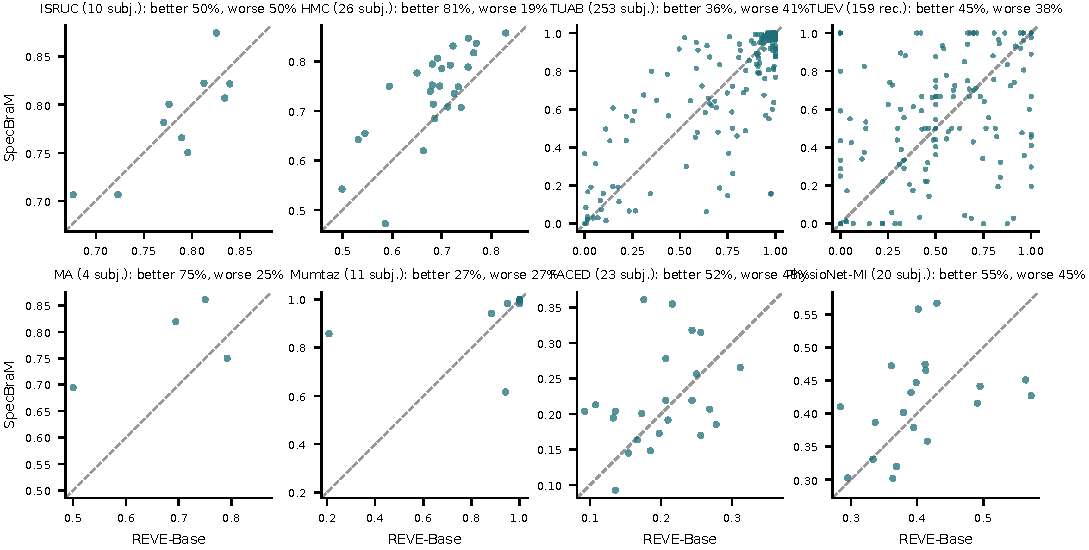
\includegraphics[width=\textwidth]{figures/per_subject.pdf}
\caption{\textbf{Per-subject balanced accuracy}, SpecBraM's main checkpoint vs.\ REVE-Base
(strict linear probe; one point per test subject, TUEV: per recording; dashed: equality).
Titles: share of subjects on which SpecBraM is better / worse.}
\label{fig:per_subject}
\end{figure*}
% auto-generated by make_case_figs.py -- do not edit
\begin{table}[h]\centering\small
\setlength{\tabcolsep}{3pt}
\caption{\textbf{Per-subject comparison}: percentage of test subjects (TUEV: recordings) on
which SpecBraM's balanced accuracy is higher / equal / lower than that of each external model
(strict linear probe, one checkpoint per model).}
\label{tab:per_subject}
\resizebox{\columnwidth}{!}{%
\begin{tabular}{l ccccc}
\toprule
Dataset & CBraMod & LaBraM-Base & BIOT & CSBrain & REVE-Base \\
\midrule
ISRUC (10 subj.) & 100/0/0 & 90/0/10 & 90/0/10 & 100/0/0 & 50/0/50 \\
HMC (26 subj.) & 100/0/0 & 96/0/4 & 96/0/4 & 100/0/0 & 81/0/19 \\
TUAB (253 subj.) & 60/13/27 & 65/10/25 & -- & 62/11/27 & 36/23/41 \\
TUEV (159 rec.) & 50/17/33 & 50/19/31 & -- & 45/21/34 & 45/18/37 \\
MA (4 subj.) & 75/0/25 & 100/0/0 & -- & 100/0/0 & 75/0/25 \\
Mumtaz (11 subj.) & 45/36/19 & 64/27/9 & -- & 82/18/0 & 27/45/28 \\
FACED (23 subj.) & 78/0/22 & 83/0/17 & -- & 65/0/35 & 52/0/48 \\
PhysioNet-MI (20 subj.) & 85/0/15 & 95/0/5 & -- & 90/0/10 & 55/0/45 \\
\bottomrule
\end{tabular}}
\end{table}


\subsection{Sleep Staging: ISRUC}
ISRUC subgroup~I \cite{khalighi2016isruc} contains one overnight polysomnography of each of
100 adults with sleep complaints, scored by experts in 30-s epochs into five AASM stages (W, N1,
N2, N3, REM). We use the six mastoid-referenced EEG leads (F3-A2, C3-A2, O1-A2, F4-A1, C4-A1,
O2-A1; 200\,Hz), of which F3/F4 are missing in some recordings, and the subject split of CBraMod
and CSBrain (subjects 1--80/81--90/91--100; 71{,}936/9{,}438/8{,}813 epochs). A 30-s epoch is represented by
the mean of the features of its three 10-s windows.
% auto-generated by make_arxiv_tables.py -- do not edit
\begin{table}[h]\centering\small
\setlength{\tabcolsep}{3pt}
\caption{\textbf{Detailed results on ISRUC} (strict linear probe). One checkpoint
per model, with the 95\% confidence interval from 1{,}000 bootstrap resamples of the
10 test subjects. Below SpecBraM's main
checkpoint: mean${\pm}$std over its three pretraining seeds. Bold: best per column.}
\label{tab:det_isruc}
\resizebox{\columnwidth}{!}{%
\begin{tabular}{l ccc}
\toprule
Model & Balanced Acc. & Cohen's $\kappa$ & Weighted F1\\
\midrule
\textbf{SpecBraM} & \ci{0.790}{0.764}{0.816} & \ci{0.733}{0.692}{0.773} & \ci{\textbf{0.795}}{0.757}{0.830} \\
\quad{\footnotesize three seeds, mean${\pm}$std} & \val{0.797}{0.006} & \val{0.744}{0.010} & \val{0.803}{0.008} \\
CBraMod & \ci{0.728}{0.702}{0.752} & \ci{0.658}{0.608}{0.705} & \ci{0.734}{0.698}{0.770} \\
LaBraM-Base & \ci{0.752}{0.720}{0.777} & \ci{0.686}{0.642}{0.724} & \ci{0.754}{0.716}{0.787} \\
BIOT & \ci{0.736}{0.691}{0.771} & \ci{0.666}{0.601}{0.715} & \ci{0.740}{0.686}{0.785} \\
CSBrain & \ci{0.730}{0.706}{0.752} & \ci{0.674}{0.638}{0.714} & \ci{0.749}{0.719}{0.782} \\
REVE-Base & \ci{\textbf{0.793}}{0.765}{0.816} & \ci{\textbf{0.736}}{0.703}{0.769} & \ci{\textbf{0.795}}{0.765}{0.824} \\
\bottomrule
\end{tabular}}
\end{table}

\begin{figure}[h]\centering
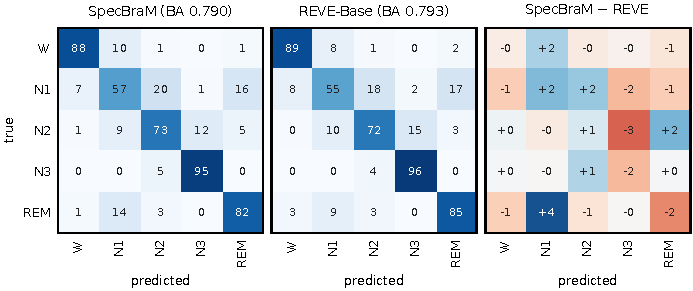
\includegraphics[width=\columnwidth]{figures/cm_isruc.pdf}
\caption{\textbf{Confusion matrices on ISRUC} (strict linear probe, row-normalized recall in \%): SpecBraM's main checkpoint, REVE-Base and their difference (blue: SpecBraM higher).}
\label{fig:cm_isruc}
\end{figure}
Fig.~\ref{fig:cm_isruc}: The two models make the same kinds of errors: N1 is confused with N2 and REM, and N3 with N2. Per-class recall differs by at most $2.4$ points, consistent with the small difference in balanced-accuracy point estimates.

\subsection{Sleep Staging: HMC}
HMC \cite{alvarez2021hmc} contains 151 clinical polysomnographies from the Haaglanden Medisch
Centrum, scored in 30-s epochs into the same five stages. We use the four EEG leads (F4-M1,
C4-M1, O2-M1, C3-M2; 256\,Hz) and the split of CBraMod and CSBrain by sorted subject ID
(100/25/26 recordings; 91{,}248/22{,}124/23{,}871 epochs). Epochs are represented as for ISRUC.
% auto-generated by make_arxiv_tables.py -- do not edit
\begin{table}[h]\centering\small
\setlength{\tabcolsep}{3pt}
\caption{\textbf{Detailed results on HMC} (strict linear probe). One checkpoint
per model, with the 95\% confidence interval from 1{,}000 bootstrap resamples of the
26 test subjects. Below SpecBraM's main
checkpoint: mean${\pm}$std over its three pretraining seeds. Bold: best per column.}
\label{tab:det_hmc}
\resizebox{\columnwidth}{!}{%
\begin{tabular}{l ccc}
\toprule
Model & Balanced Acc. & Cohen's $\kappa$ & Weighted F1\\
\midrule
\textbf{SpecBraM} & \ci{\textbf{0.742}}{0.699}{0.776} & \ci{\textbf{0.675}}{0.620}{0.724} & \ci{\textbf{0.751}}{0.707}{0.791} \\
\quad{\footnotesize three seeds, mean${\pm}$std} & \val{0.743}{0.002} & \val{0.675}{0.002} & \val{0.749}{0.003} \\
CBraMod & \ci{0.619}{0.576}{0.654} & \ci{0.513}{0.459}{0.567} & \ci{0.619}{0.572}{0.665} \\
LaBraM-Base & \ci{0.632}{0.583}{0.673} & \ci{0.530}{0.473}{0.585} & \ci{0.636}{0.586}{0.680} \\
BIOT & \ci{0.658}{0.609}{0.697} & \ci{0.562}{0.507}{0.615} & \ci{0.661}{0.616}{0.704} \\
CSBrain & \ci{0.611}{0.580}{0.641} & \ci{0.515}{0.472}{0.554} & \ci{0.625}{0.590}{0.660} \\
REVE-Base & \ci{0.704}{0.664}{0.737} & \ci{0.623}{0.577}{0.670} & \ci{0.707}{0.671}{0.745} \\
\bottomrule
\end{tabular}}
\end{table}

\begin{figure}[h]\centering
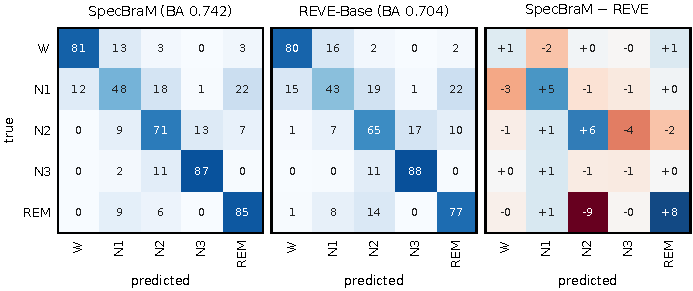
\includegraphics[width=\columnwidth]{figures/cm_hmc.pdf}
\caption{\textbf{Confusion matrices on HMC} (strict linear probe, row-normalized recall in \%): SpecBraM's main checkpoint, REVE-Base and their difference (blue: SpecBraM higher).}
\label{fig:cm_hmc}
\end{figure}
Fig.~\ref{fig:cm_hmc}: SpecBraM's lead over REVE comes from the transitional and REM stages: its recall is higher by $5.0$ points for N1, $6.0$ for N2 and $7.7$ for REM, while W and N3, the stages with the most distinct spectra, are recognized equally well by both.

\noindent\textbf{Case study: one night per dataset.} Fig.~\ref{fig:hypnogram} shows the
hypnograms of one test subject per sleep dataset, chosen by rule as the subject whose SpecBraM
balanced accuracy is closest to the median of its dataset, with the stages predicted by
SpecBraM, REVE and CBraMod from the frozen features of each 30-s epoch alone (no sequence
model). All models follow the sleep cycles; their errors concentrate at stage transitions and in
N1. On the ISRUC night the three models are close (balanced accuracy $0.800$, $0.776$ and $0.728$).
On the HMC night SpecBraM reaches $0.750$ against $0.594$ for REVE, which scores almost a third
of the N2 epochs as N3 (99 of 319 vs.\ 27 for SpecBraM) and half of the REM epochs as N2 (69 of
132 vs.\ 12), the same errors that dominate REVE's confusion matrix on the whole dataset
(Fig.~\ref{fig:cm_hmc}).
\begin{figure*}[t]\centering
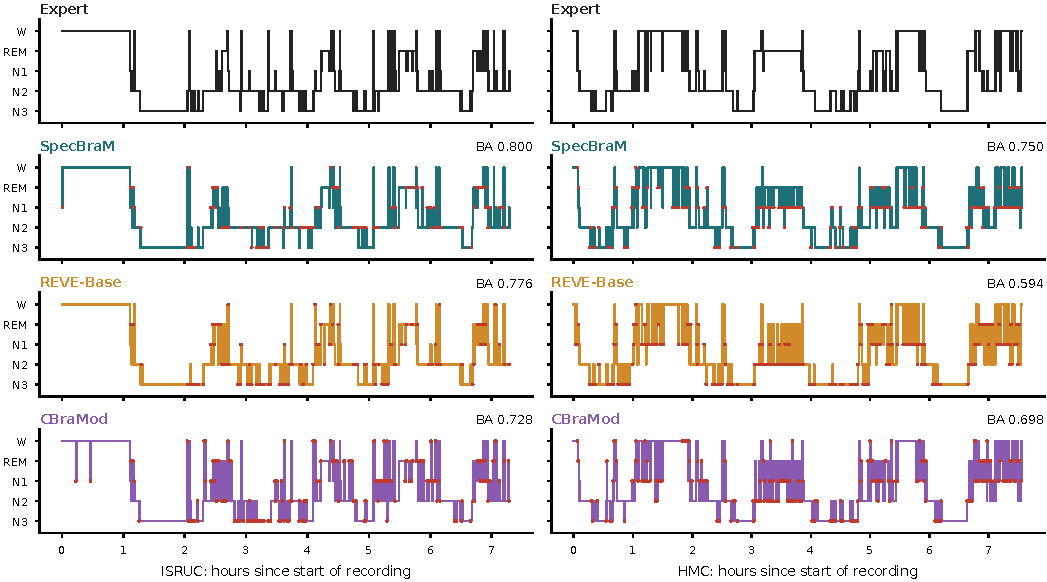
\includegraphics[width=\textwidth]{figures/hypnogram.pdf}
\caption{\textbf{Whole-night hypnograms} of one test subject per sleep dataset (left: ISRUC,
right: HMC; the subject whose SpecBraM balanced accuracy is closest to the dataset median).
Top: expert scoring; below: stages predicted by the strict linear probe on each model's frozen
features, epoch by epoch. Red dots: errors.}
\label{fig:hypnogram}
\end{figure*}

\subsection{Abnormal EEG Detection: TUAB}
TUAB \cite{obeid2016tuh} contains clinical EEG recordings of the Temple University Hospital
labeled normal or abnormal by neurologists. Following CBraMod, recordings are resampled to
200\,Hz, filtered (0.3--75\,Hz, 60\,Hz notch), converted to 16 bipolar channels of the TCP
montage and cut into non-overlapping 10-s windows that inherit the recording label. The official
evaluation folder is the test set; the training folder is split 80/20 by sorted patient ID
within each class (297{,}103/75{,}407/36{,}945 windows). The prepared metadata show three patients shared
between training and validation under this original per-class split. Test patients are disjoint
from both training and validation. All models use these same samples and splits; the overlap
limits validation independence. This downstream split issue is separate from possible TUEG
pretraining overlap.
% auto-generated by make_arxiv_tables.py -- do not edit
\begin{table*}[t]\centering\small
\setlength{\tabcolsep}{8pt}
\caption{\textbf{Detailed results on TUAB} (strict linear probe). One checkpoint
per model, with the 95\% confidence interval from 1{,}000 bootstrap resamples of the
253 test subjects. Below SpecBraM's main
checkpoint: mean${\pm}$std over its three pretraining seeds. Bold: best per column.}
\label{tab:det_tuab}

\begin{tabular}{l ccccc}
\toprule
Model & Balanced Acc. & Cohen's $\kappa$ & Weighted F1 & AUROC & AUC-PR\\
\midrule
\textbf{SpecBraM} & \ci{0.813}{0.775}{0.850} & \ci{0.627}{0.554}{0.700} & \ci{0.815}{0.778}{0.851} & \ci{\textbf{0.891}}{0.851}{0.924} & \ci{0.897}{0.860}{0.929} \\
\quad{\footnotesize three seeds, mean${\pm}$std} & \val{0.805}{0.007} & \val{0.611}{0.014} & \val{0.807}{0.007} & \val{0.880}{0.011} & \val{0.890}{0.008} \\
CBraMod & \ci{0.778}{0.738}{0.814} & \ci{0.558}{0.480}{0.629} & \ci{0.780}{0.742}{0.816} & \ci{0.856}{0.810}{0.894} & \ci{0.857}{0.812}{0.893} \\
LaBraM-Base & \ci{0.776}{0.740}{0.812} & \ci{0.554}{0.484}{0.624} & \ci{0.779}{0.744}{0.814} & \ci{0.856}{0.817}{0.891} & \ci{0.851}{0.806}{0.889} \\
CSBrain & \ci{0.772}{0.736}{0.805} & \ci{0.546}{0.475}{0.611} & \ci{0.774}{0.740}{0.807} & \ci{0.845}{0.804}{0.882} & \ci{0.836}{0.786}{0.878} \\
REVE-Base & \ci{\textbf{0.821}}{0.781}{0.861} & \ci{\textbf{0.644}}{0.565}{0.722} & \ci{\textbf{0.823}}{0.784}{0.861} & \ci{0.889}{0.848}{0.925} & \ci{\textbf{0.902}}{0.864}{0.933} \\
\bottomrule
\end{tabular}
\end{table*}

\begin{figure}[h]\centering
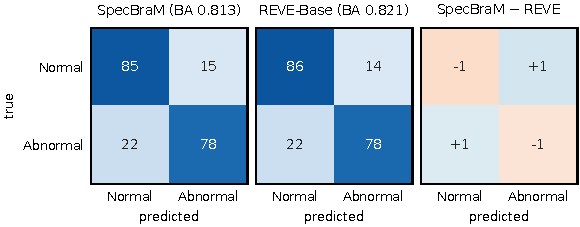
\includegraphics[width=\columnwidth]{figures/cm_tuab.pdf}
\caption{\textbf{Confusion matrices on TUAB} (strict linear probe, row-normalized recall in \%): SpecBraM's main checkpoint, REVE-Base and their difference (blue: SpecBraM higher).}
\label{fig:cm_tuab}
\end{figure}
Fig.~\ref{fig:cm_tuab}: Both models recognize normal and abnormal recordings almost equally well (recall within one point of each other); REVE's slightly higher balanced accuracy is spread over both classes.

\subsection{Event Classification: TUEV}
TUEV \cite{obeid2016tuh} annotates clinical EEG with six event classes: spike and sharp wave
(SPSW), generalized and lateralized periodic epileptiform discharges (GPED, PLED), eye movement
(EYEM), artifact (ARTF) and background (BCKG). Following CBraMod, each annotated 1-s event is
represented by a 5-s window centred on it, with the same filtering and 16-channel bipolar
montage as TUAB. The official evaluation folder is the test set and the training folder is split
80/20 by sorted patient ID (68{,}445/15{,}487/29{,}421 windows), with no patient overlap among the three
downstream splits. Background makes up 65\% of the windows; Cohen's
$\kappa$ and weighted F1 are dominated by it, whereas balanced accuracy weights the rare
epileptiform classes equally. This explains why REVE has the highest $\kappa$ and weighted F1
here although its balanced accuracy is below SpecBraM's and CSBrain's.
% auto-generated by make_arxiv_tables.py -- do not edit
\begin{table}[h]\centering\small
\setlength{\tabcolsep}{3pt}
\caption{\textbf{Detailed results on TUEV} (strict linear probe). One checkpoint
per model, with the 95\% confidence interval from 1{,}000 bootstrap resamples of the
159 test recordings. Below SpecBraM's main
checkpoint: mean${\pm}$std over its three pretraining seeds. Bold: best per column.}
\label{tab:det_tuev}
\resizebox{\columnwidth}{!}{%
\begin{tabular}{l ccc}
\toprule
Model & Balanced Acc. & Cohen's $\kappa$ & Weighted F1\\
\midrule
\textbf{SpecBraM} & \ci{0.555}{0.491}{0.648} & \ci{0.467}{0.369}{0.557} & \ci{0.722}{0.659}{0.777} \\
\quad{\footnotesize three seeds, mean${\pm}$std} & \val{0.561}{0.025} & \val{0.474}{0.049} & \val{0.724}{0.027} \\
CBraMod & \ci{0.525}{0.471}{0.609} & \ci{0.399}{0.327}{0.480} & \ci{0.669}{0.598}{0.742} \\
LaBraM-Base & \ci{0.468}{0.416}{0.545} & \ci{0.327}{0.228}{0.423} & \ci{0.624}{0.518}{0.710} \\
CSBrain & \ci{\textbf{0.564}}{0.505}{0.621} & \ci{0.421}{0.348}{0.489} & \ci{0.683}{0.619}{0.745} \\
REVE-Base & \ci{0.546}{0.500}{0.587} & \ci{\textbf{0.566}}{0.439}{0.655} & \ci{\textbf{0.778}}{0.727}{0.820} \\
\bottomrule
\end{tabular}}
\end{table}

\begin{figure}[h]\centering
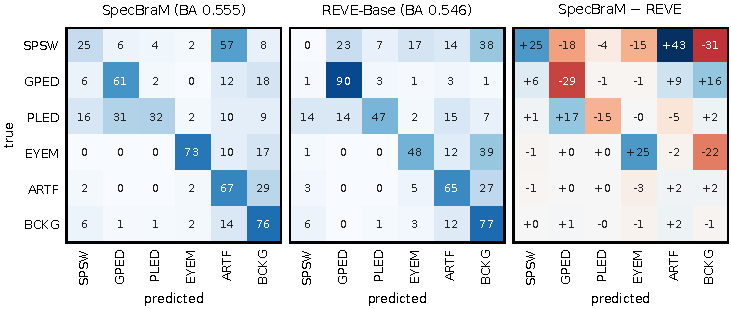
\includegraphics[width=\columnwidth]{figures/cm_tuev.pdf}
\caption{\textbf{Confusion matrices on TUEV} (strict linear probe, row-normalized recall in \%): SpecBraM's main checkpoint, REVE-Base and their difference (blue: SpecBraM higher).}
\label{fig:cm_tuev}
\end{figure}
Fig.~\ref{fig:cm_tuev}: The two models differ in kind. SpecBraM detects spike and sharp waves
(SPSW recall $25\%$ vs.\ $0\%$; REVE never predicts this class) and eye movements ($73\%$ vs.\
$48\%$), events with a distinct spectral signature. REVE is better on the periodic discharges
(GPED $90\%$ vs.\ $61\%$, PLED $47\%$ vs.\ $32\%$), which involve waveform shape and repetition
over seconds. This pattern is consistent with P4, but the models also differ in architecture
and pretraining data, so it does not isolate the effect of phase invariance.

\noindent\textbf{Examples.} Fig.~\ref{fig:tuev_cases} shows four test windows on which the two
models disagree, chosen by rule: for each class, the window that the correct model classifies
with the highest confidence. SpecBraM recognizes a spike and sharp wave that REVE labels as a
lateralized periodic discharge, and an eye-movement window that REVE labels as background. REVE
recognizes a generalized and a lateralized periodic discharge that SpecBraM labels as
background. In the GPED window the discharges recur about every two seconds across all
channels. Their waveform and repetition extend beyond the band power of a single 0.78-s patch.
The patch-local target does not directly supervise this longer temporal pattern (P4), although
the encoder can still represent temporal and waveform information.
\begin{figure*}[t]\centering
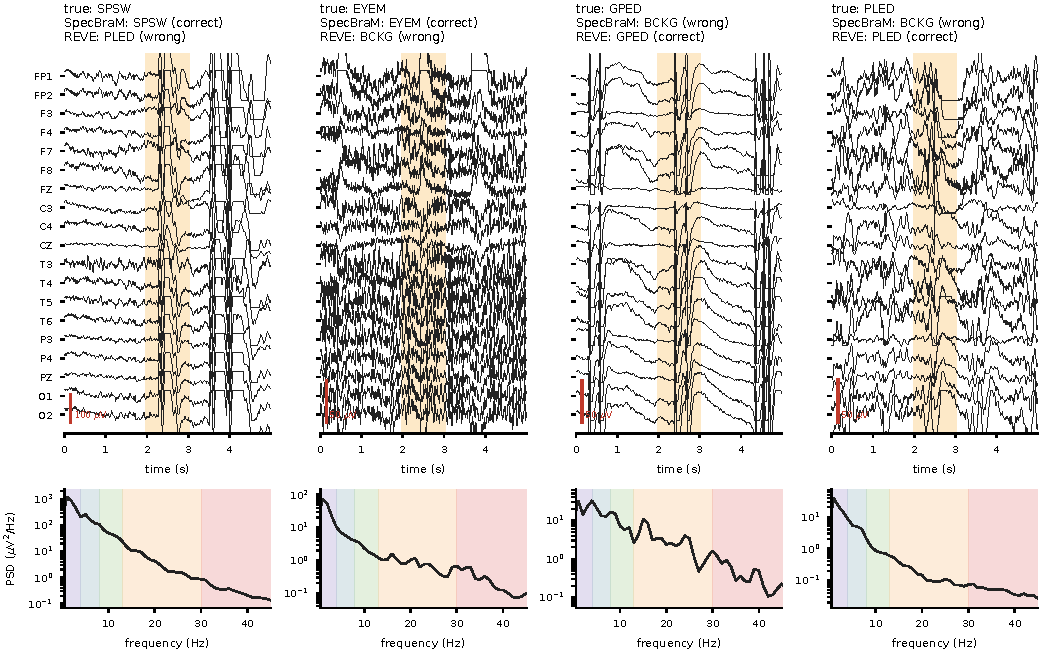
\includegraphics[width=\textwidth]{figures/tuev_cases.pdf}
\caption{\textbf{TUEV examples on which SpecBraM and REVE disagree} (strict linear probe; for
each class the window that the correct model classifies most confidently). Top: the 5-s window
(19 monopolar leads, CBraMod's preprocessing; shaded: the annotated 1-s event; traces clipped to
their row). Bottom: power spectral density averaged over channels, with the five bands of the
target.}
\label{fig:tuev_cases}
\end{figure*}

\subsection{Mental Workload: MA}
The mental arithmetic dataset \cite{zyma2019mentalarith} records 36 subjects at rest and during
serial subtraction with 20 leads (19 standard 10--20 leads and A2-A1; 500\,Hz). Following
CBraMod, recordings are resampled to 200\,Hz and cut into 5-s windows labeled rest or task, and
the sorted subjects are split 28/4/4 (1{,}343/172/192 windows). With four test subjects, MA has by far
the widest confidence intervals of all tasks.
% auto-generated by make_arxiv_tables.py -- do not edit
\begin{table*}[t]\centering\small
\setlength{\tabcolsep}{8pt}
\caption{\textbf{Detailed results on MA} (strict linear probe). One checkpoint
per model, with the 95\% confidence interval from 1{,}000 bootstrap resamples of the
4 test subjects. Below SpecBraM's main
checkpoint: mean${\pm}$std over its three pretraining seeds. Bold: best per column.}
\label{tab:det_ma}

\begin{tabular}{l ccccc}
\toprule
Model & Balanced Acc. & Cohen's $\kappa$ & Weighted F1 & AUROC & AUC-PR\\
\midrule
\textbf{SpecBraM} & \ci{\textbf{0.781}}{0.722}{0.840} & \ci{\textbf{0.583}}{0.526}{0.655} & \ci{\textbf{0.846}}{0.817}{0.876} & \ci{\textbf{0.912}}{0.878}{0.981} & \ci{\textbf{0.783}}{0.751}{0.942} \\
\quad{\footnotesize three seeds, mean${\pm}$std} & \val{0.747}{0.030} & \val{0.500}{0.093} & \val{0.810}{0.047} & \val{0.861}{0.052} & \val{0.706}{0.108} \\
CBraMod & \ci{0.653}{0.507}{0.799} & \ci{0.256}{0.011}{0.510} & \ci{0.686}{0.525}{0.811} & \ci{0.708}{0.532}{0.884} & \ci{0.515}{0.305}{0.730} \\
LaBraM-Base & \ci{0.681}{0.597}{0.736} & \ci{0.342}{0.205}{0.452} & \ci{0.746}{0.700}{0.793} & \ci{0.734}{0.649}{0.834} & \ci{0.571}{0.432}{0.724} \\
CSBrain & \ci{0.556}{0.403}{0.653} & \ci{0.095}{-0.175}{0.275} & \ci{0.626}{0.543}{0.711} & \ci{0.586}{0.402}{0.747} & \ci{0.306}{0.218}{0.451} \\
REVE-Base & \ci{0.684}{0.562}{0.771} & \ci{0.361}{0.143}{0.551} & \ci{0.758}{0.679}{0.838} & \ci{0.757}{0.669}{0.924} & \ci{0.587}{0.485}{0.802} \\
\bottomrule
\end{tabular}
\end{table*}

\begin{figure}[h]\centering
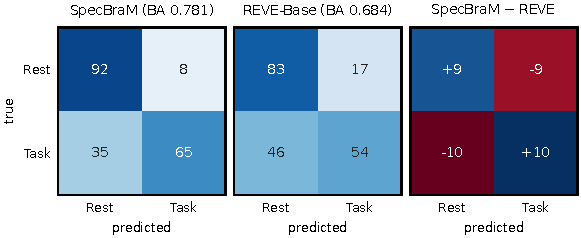
\includegraphics[width=\columnwidth]{figures/cm_ma.pdf}
\caption{\textbf{Confusion matrices on MA} (strict linear probe, row-normalized recall in \%): SpecBraM's main checkpoint, REVE-Base and their difference (blue: SpecBraM higher).}
\label{fig:cm_ma}
\end{figure}
Fig.~\ref{fig:cm_ma}: SpecBraM is better on both conditions (rest $+9.0$, task $+10.4$ points recall), so its lead is not a shift of the decision threshold.

\subsection{Depression: Mumtaz}
Mumtaz \cite{mumtaz2016mdd} contains resting-state EEG (eyes open and closed) of patients with
major depressive disorder and healthy controls, recorded with 19 linked-ear-referenced leads at
256\,Hz. Following CBraMod, recordings are resampled to 200\,Hz, filtered (0.3--75\,Hz, 50\,Hz
notch) and cut into 5-s windows that inherit the subject's diagnosis; recordings are split by
subject within each group (4{,}891/1{,}041/1{,}211 windows).
% auto-generated by make_arxiv_tables.py -- do not edit
\begin{table*}[t]\centering\small
\setlength{\tabcolsep}{8pt}
\caption{\textbf{Detailed results on Mumtaz} (strict linear probe). One checkpoint
per model, with the 95\% confidence interval from 1{,}000 bootstrap resamples of the
11 test subjects. Below SpecBraM's main
checkpoint: mean${\pm}$std over its three pretraining seeds. Bold: best per column.}
\label{tab:det_mumtaz}

\begin{tabular}{l ccccc}
\toprule
Model & Balanced Acc. & Cohen's $\kappa$ & Weighted F1 & AUROC & AUC-PR\\
\midrule
\textbf{SpecBraM} & \ci{\textbf{0.939}}{0.868}{0.995} & \ci{\textbf{0.879}}{0.733}{0.991} & \ci{\textbf{0.940}}{0.865}{0.995} & \ci{\textbf{0.991}}{0.964}{1.000} & \ci{\textbf{0.991}}{0.967}{1.000} \\
\quad{\footnotesize three seeds, mean${\pm}$std} & \val{0.942}{0.007} & \val{0.884}{0.015} & \val{0.942}{0.007} & \val{0.994}{0.003} & \val{0.994}{0.003} \\
CBraMod & \ci{0.893}{0.760}{0.988} & \ci{0.787}{0.513}{0.978} & \ci{0.893}{0.744}{0.989} & \ci{0.973}{0.911}{1.000} & \ci{0.973}{0.908}{1.000} \\
LaBraM-Base & \ci{0.876}{0.744}{0.986} & \ci{0.754}{0.484}{0.974} & \ci{0.877}{0.735}{0.987} & \ci{0.963}{0.882}{0.999} & \ci{0.960}{0.874}{0.999} \\
CSBrain & \ci{0.864}{0.774}{0.943} & \ci{0.727}{0.549}{0.887} & \ci{0.864}{0.772}{0.944} & \ci{0.947}{0.878}{0.990} & \ci{0.942}{0.862}{0.987} \\
REVE-Base & \ci{0.902}{0.743}{0.994} & \ci{0.804}{0.481}{0.989} & \ci{0.901}{0.728}{0.995} & \ci{0.968}{0.879}{1.000} & \ci{0.963}{0.861}{1.000} \\
\bottomrule
\end{tabular}
\end{table*}

\begin{figure}[h]\centering
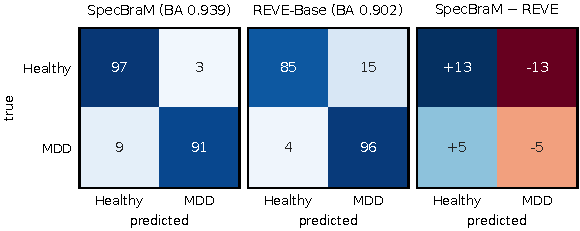
\includegraphics[width=\columnwidth]{figures/cm_mumtaz.pdf}
\caption{\textbf{Confusion matrices on Mumtaz} (strict linear probe, row-normalized recall in \%): SpecBraM's main checkpoint, REVE-Base and their difference (blue: SpecBraM higher).}
\label{fig:cm_mumtaz}
\end{figure}
Fig.~\ref{fig:cm_mumtaz}: SpecBraM's gain comes from fewer healthy subjects classified as depressed (recall of the healthy class $+12.6$ points), at a cost of $5.2$ points on the depressed class.

\subsection{Emotion Recognition: FACED}
FACED \cite{chen2023faced} records 123 subjects watching 28 video clips that elicit nine emotion
categories (anger, disgust, fear, sadness, neutral, amusement, inspiration, joy, tenderness),
with 32 leads at 250\,Hz. The last 30\,s of each clip are resampled to 200\,Hz and cut into three
10-s windows labeled with the clip's category; the sorted subjects are split 80/20/23
(6{,}720/1{,}680/1{,}932 windows; chance level $1/9$).
% auto-generated by make_arxiv_tables.py -- do not edit
\begin{table}[h]\centering\small
\setlength{\tabcolsep}{3pt}
\caption{\textbf{Detailed results on FACED} (strict linear probe). One checkpoint
per model, with the 95\% confidence interval from 1{,}000 bootstrap resamples of the
23 test subjects. Below SpecBraM's main
checkpoint: mean${\pm}$std over its three pretraining seeds. Bold: best per column.}
\label{tab:det_faced}
\resizebox{\columnwidth}{!}{%
\begin{tabular}{l ccc}
\toprule
Model & Balanced Acc. & Cohen's $\kappa$ & Weighted F1\\
\midrule
\textbf{SpecBraM} & \ci{\textbf{0.221}}{0.195}{0.248} & \ci{\textbf{0.126}}{0.096}{0.155} & \ci{\textbf{0.219}}{0.193}{0.245} \\
\quad{\footnotesize three seeds, mean${\pm}$std} & \val{0.216}{0.013} & \val{0.119}{0.015} & \val{0.214}{0.010} \\
CBraMod & \ci{0.171}{0.156}{0.188} & \ci{0.069}{0.052}{0.087} & \ci{0.167}{0.151}{0.182} \\
LaBraM-Base & \ci{0.167}{0.152}{0.181} & \ci{0.064}{0.047}{0.079} & \ci{0.163}{0.144}{0.177} \\
CSBrain & \ci{0.179}{0.161}{0.199} & \ci{0.077}{0.057}{0.098} & \ci{0.171}{0.153}{0.189} \\
REVE-Base & \ci{0.200}{0.179}{0.225} & \ci{0.101}{0.076}{0.130} & \ci{0.200}{0.177}{0.224} \\
\bottomrule
\end{tabular}}
\end{table}

\begin{figure*}[t]\centering
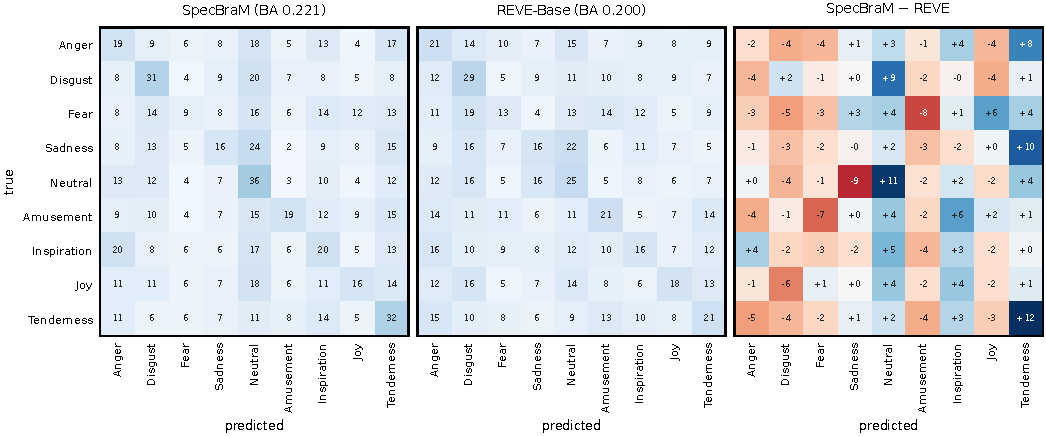
\includegraphics[width=\textwidth]{figures/cm_faced.pdf}
\caption{\textbf{Confusion matrices on FACED} (strict linear probe, row-normalized recall in \%): SpecBraM's main checkpoint, REVE-Base and their difference (blue: SpecBraM higher).}
\label{fig:cm_faced}
\end{figure*}
Fig.~\ref{fig:cm_faced}: Both models are far from perfect on nine emotions. SpecBraM's gain is concentrated on neutral ($+11.2$ points) and tenderness ($+11.6$), the two categories at the low-arousal end, while the other categories differ by a few points in either direction.

\subsection{Motor Imagery: PhysioNet-MI}
PhysioNet-MI \cite{schalk2004bci2000} records 109 subjects with 64 leads at 160\,Hz while they
imagine opening and closing the left fist, the right fist, both fists or both feet. Following
CBraMod, the imagery runs are high-pass filtered at 0.3\,Hz, notch filtered at 60\,Hz and
resampled to 200\,Hz, and the 4-s window after each cue is labeled with the imagined movement;
the sorted subjects are split 70/19/20 (6{,}300/1{,}734/1{,}803 windows; chance level $1/4$).
% auto-generated by make_arxiv_tables.py -- do not edit
\begin{table}[h]\centering\small
\setlength{\tabcolsep}{3pt}
\caption{\textbf{Detailed results on PhysioNet-MI} (strict linear probe). One checkpoint
per model, with the 95\% confidence interval from 1{,}000 bootstrap resamples of the
20 test subjects. Below SpecBraM's main
checkpoint: mean${\pm}$std over its three pretraining seeds. Bold: best per column.}
\label{tab:det_physio}
\resizebox{\columnwidth}{!}{%
\begin{tabular}{l ccc}
\toprule
Model & Balanced Acc. & Cohen's $\kappa$ & Weighted F1\\
\midrule
\textbf{SpecBraM} & \ci{\textbf{0.417}}{0.384}{0.450} & \ci{\textbf{0.223}}{0.179}{0.267} & \ci{\textbf{0.416}}{0.383}{0.449} \\
\quad{\footnotesize three seeds, mean${\pm}$std} & \val{0.397}{0.018} & \val{0.196}{0.024} & \val{0.396}{0.018} \\
CBraMod & \ci{0.312}{0.286}{0.340} & \ci{0.083}{0.048}{0.119} & \ci{0.310}{0.282}{0.337} \\
LaBraM-Base & \ci{0.299}{0.285}{0.314} & \ci{0.065}{0.047}{0.085} & \ci{0.299}{0.282}{0.312} \\
CSBrain & \ci{0.298}{0.273}{0.325} & \ci{0.064}{0.030}{0.100} & \ci{0.295}{0.270}{0.320} \\
REVE-Base & \ci{0.403}{0.371}{0.438} & \ci{0.204}{0.161}{0.250} & \ci{0.403}{0.371}{0.437} \\
\bottomrule
\end{tabular}}
\end{table}

\begin{figure}[h]\centering
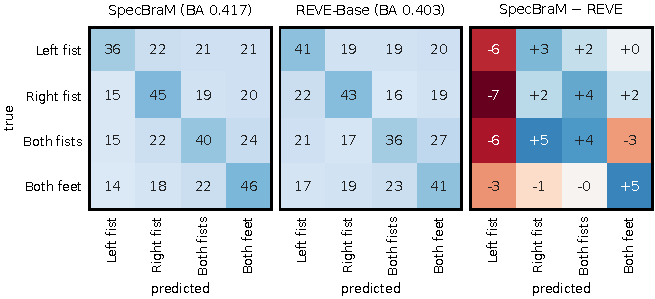
\includegraphics[width=\columnwidth]{figures/cm_physio.pdf}
\caption{\textbf{Confusion matrices on PhysioNet-MI} (strict linear probe, row-normalized recall in \%): SpecBraM's main checkpoint, REVE-Base and their difference (blue: SpecBraM higher).}
\label{fig:cm_physio}
\end{figure}
Fig.~\ref{fig:cm_physio}: SpecBraM is better on bilateral imagery (both fists $+4.2$, both feet $+4.9$ points) and slightly worse on the left fist ($-5.5$); distinguishing the left and right fist requires lateralized spatial patterns that a mean-pooled readout dilutes.


\section{Band Power versus Waveform Reconstruction beyond Sleep}\label{app:targettasks}
% auto-generated by make_arxiv_tables.py -- do not edit
\begin{table}[t]\centering\small
\setlength{\tabcolsep}{2.5pt}
\caption{\textbf{Band power vs.\ raw-waveform reconstruction beyond sleep} (same architecture,
data and steps; strict linear probe, balanced accuracy, mean${\pm}$std over three pretraining
seeds). Bold: best per column.}
\label{tab:target_tasks}
\resizebox{\columnwidth}{!}{%
\begin{tabular}{l cccccc}
\toprule
Target & TUAB & TUEV & MA & Mumtaz & FACED & PhysioNet-MI\\
\midrule
\textbf{Band power} (ours) & \val{\textbf{0.805}}{0.007} & \val{\textbf{0.561}}{0.025} & \val{\textbf{0.747}}{0.030} & \val{\textbf{0.942}}{0.007} & \val{0.216}{0.013} & \val{\textbf{0.397}}{0.018} \\
Raw-waveform reconstruction & \val{0.804}{0.002} & \val{0.533}{0.027} & \val{0.685}{0.051} & \val{0.924}{0.013} & \val{\textbf{0.220}}{0.010} & \val{0.395}{0.013} \\
\bottomrule
\end{tabular}}
\end{table}

Table~\ref{tab:target_tasks} extends the target study of Sec.~\ref{sec:targetstudy} to the other
tasks. Band power has higher mean scores on mental arithmetic ($+6.2$), depression screening
($+1.8$) and event classification ($+2.8$), and close mean scores on emotion recognition, motor
imagery and abnormality detection; these comparisons do not establish equivalence.

\section{Fine-Tuning}\label{app:fttasks}
% auto-generated by make_arxiv_tables.py -- do not edit
\begin{table*}[t]\centering\footnotesize
\setlength{\tabcolsep}{3pt}
\caption{\textbf{Sleep staging, fine-tuned} (5-class, 30-s epochs in sequences of 20, one
shared 1-layer sequence transformer; identical subject-disjoint splits as
\citet{csbrain}). Baselines as reported by \citet{csbrain} (REVE: its paper, ISRUC only).
Our rows: mean${\pm}$std over three \emph{pretraining} seeds (one fine-tuning run each), so
the spread includes pretraining variance, unlike the baselines' fine-tuning-seed spread.
Bold: best per column.}
\label{tab:ft30}
\resizebox{\textwidth}{!}{%
\begin{tabular}{l c ccc ccc}
\toprule
& & \multicolumn{3}{c}{ISRUC} & \multicolumn{3}{c}{HMC}\\
\cmidrule(lr){3-5}\cmidrule(lr){6-8}
Method & Pretrain (h) & BA & $\kappa$ & Weighted F1 & BA & $\kappa$ & Weighted F1\\
\midrule
\multicolumn{8}{l}{\emph{Task-specific models}}\\
EEGNet~\cite{lawhern2018eegnet} & -- & \val{0.7154}{0.0121} & \val{0.7040}{0.0173} & \val{0.7513}{0.0124} & \val{0.6534}{0.0122} & \val{0.5886}{0.0201} & \val{0.6536}{0.0168} \\
EEGConformer~\cite{song2023conformer} & -- & \val{0.7400}{0.0133} & \val{0.7143}{0.0162} & \val{0.7634}{0.0151} & \val{0.7149}{0.0086} & \val{0.6432}{0.0055} & \val{0.7080}{0.0039} \\
SPaRCNet~\cite{jing2023sparcnet} & -- & \val{0.7487}{0.0075} & \val{0.7097}{0.0132} & \val{0.7624}{0.0092} & \val{0.4756}{0.1109} & \val{0.3147}{0.1315} & \val{0.4108}{0.1310} \\
ContraWR~\cite{yang2023contrawr} & -- & \val{0.7402}{0.0126} & \val{0.7178}{0.0156} & \val{0.7610}{0.0137} & \val{0.4242}{0.0541} & \val{0.2340}{0.0554} & \val{0.2987}{0.0288} \\
CNN-Transformer~\cite{peh2022cnntransformer} & -- & \val{0.7363}{0.0087} & \val{0.7129}{0.0121} & \val{0.7719}{0.0153} & \val{0.6573}{0.0141} & \val{0.5961}{0.0105} & \val{0.6896}{0.0065} \\
FFCL~\cite{li2022ffcl} & -- & \val{0.7277}{0.0182} & \val{0.7016}{0.0292} & \val{0.7614}{0.0197} & \val{0.4427}{0.0702} & \val{0.2542}{0.0654} & \val{0.2902}{0.0485} \\
ST-Transformer~\cite{song2021sttransformer} & -- & \val{0.7381}{0.0205} & \val{0.7013}{0.0352} & \val{0.7681}{0.0175} & \val{0.2559}{0.0141} & \val{0.0503}{0.0183} & \val{0.1428}{0.0122} \\
\midrule
\multicolumn{8}{l}{\emph{Foundation models}}\\
BIOT~\cite{yang2023biot} & mixed & \val{0.7527}{0.0121} & \val{0.7291}{0.0230} & \val{0.7790}{0.0146} & \val{0.6862}{0.0041} & \val{0.6295}{0.0113} & \val{0.7091}{0.0147} \\
LaBraM-Base~\cite{jiang2024labram} & ${\sim}2.5$k & \val{0.7633}{0.0102} & \val{0.7231}{0.0182} & \val{0.7810}{0.0133} & \val{0.7277}{0.0101} & \val{0.6813}{0.0053} & \val{0.7454}{0.0027} \\
CBraMod~\cite{wang2025cbramod} & ${\sim}9$k & \val{0.7865}{0.0110} & \val{0.7442}{0.0152} & \val{0.8011}{0.0099} & \val{0.7269}{0.0041} & \val{0.6685}{0.0104} & \val{0.7395}{0.0089} \\
CSBrain~\cite{csbrain} & ${\sim}9$k & \val{0.7925}{0.0030} & \val{0.7406}{0.0102} & \val{0.7990}{0.0091} & \val{0.7345}{0.0047} & \val{0.6818}{0.0046} & \val{0.7506}{0.0042} \\
REVE~\cite{reve2025} & ${\sim}60$k & 0.7819 & 0.7500 & 0.8005 & -- & -- & -- \\
\midrule
Raw-waveform recon.\ (same arch.) & $2{,}388$ & \val{0.8062}{0.0061} & \val{0.7519}{0.0097} & \val{0.8100}{0.0069} & \val{0.7551}{0.0079} & \val{0.6935}{0.0057} & \val{0.7631}{0.0049} \\
\textbf{SpecBraM} & $2{,}388$ & \val{\textbf{0.8177}}{0.0032} & \val{\textbf{0.7670}}{0.0070} & \val{\textbf{0.8198}}{0.0051} & \val{\textbf{0.7696}}{0.0012} & \val{\textbf{0.7151}}{0.0021} & \val{\textbf{0.7796}}{0.0024} \\
\bottomrule
\end{tabular}}
\end{table*}

\noindent\textbf{Sleep staging.} Following CBraMod and CSBrain, 30-s epochs are grouped in
sequences of 20; each epoch is encoded (mean of its three 10-s windows), and a shared one-layer
transformer predicts one stage per epoch. Encoder and head are trained with AdamW (learning
rate $10^{-4}$, weight decay $0.05$) for up to 50 epochs with early stopping on validation
balanced accuracy (patience 10). SpecBraM reaches $0.8177{\pm}0.0032$ balanced accuracy on
ISRUC and $0.7696{\pm}0.0012$ on HMC (Table~\ref{tab:ft30}), above the listed published point estimates
(CSBrain $0.7925$/$0.7345$, REVE $0.7819$ on ISRUC), with the highest Cohen's $\kappa$ on both
datasets among the listed methods. The models differ in architecture, data and training recipe, and our standard
deviations are across pretraining seeds, unlike the baselines' fine-tuning seeds. After
fine-tuning, the gap to the matched raw-reconstruction model narrows to about $1.14$/$1.45$ points
($0.8062$/$0.7551$). In these sleep experiments, the target differences are larger for frozen
and low-label probes than after full fine-tuning.

% auto-generated by make_arxiv_tables.py -- do not edit
\begin{table}[t]\centering\small
\setlength{\tabcolsep}{2.5pt}
\caption{\textbf{Full fine-tuning beyond sleep} (balanced accuracy, mean${\pm}$std over three
pretraining seeds). Same samples and splits as the linear probe; encoder and a linear head on
mean-pooled tokens are trained with layer-wise learning-rate decay, and the epoch is selected on
validation balanced accuracy. Bold: best per column.}
\label{tab:ft_tasks}
\resizebox{\columnwidth}{!}{%
\begin{tabular}{l cccccc}
\toprule
Model & MA & Mumtaz & FACED & PhysioNet-MI & TUAB & TUEV\\
\midrule
\textbf{SpecBraM} & \val{\textbf{0.740}}{0.109} & \val{0.928}{0.026} & \val{\textbf{0.276}}{0.017} & \val{\textbf{0.564}}{0.027} & \val{\textbf{0.821}}{0.004} & \val{\textbf{0.650}}{0.079} \\
Raw-waveform recon.\ (same arch.) & \val{0.670}{0.018} & \val{\textbf{0.936}}{0.006} & \val{0.273}{0.013} & \val{0.531}{0.005} & \val{0.792}{0.006} & \val{0.566}{0.025} \\
\bottomrule
\end{tabular}}
\end{table}

\noindent\textbf{Other tasks.} Table~\ref{tab:ft_tasks} fine-tunes the encoder on the non-sleep
tasks, for SpecBraM and the matched raw-reconstruction model (layer-wise learning-rate decay,
early stopping on validation balanced accuracy). Band power has higher mean scores on mental
arithmetic, motor imagery, abnormality detection and event classification, and the mean scores
are close on depression screening and emotion recognition.

\section{Variants of the Band-Power Target}\label{app:variants}
% auto-generated by make_arxiv_tables.py -- do not edit
\begin{table*}[t]\centering\small
\setlength{\tabcolsep}{4pt}
\caption{\textbf{Spectral estimator of the band-power target} (linear patch embedding; everything else as
the main model). Strict linear probe on sleep staging, mean${\pm}$std over three pretraining
seeds unless stated; columns as Table~\ref{tab:ablation}. Bold: best per column.}
\label{tab:variants}
\begin{tabular}{l cc cc cc}
\toprule
& \multicolumn{2}{c}{BA (100\% labels)} & \multicolumn{2}{c}{BA (1\% labels)} & \multicolumn{2}{c}{$\Delta$ BA (pts)}\\
\cmidrule(lr){2-3}\cmidrule(lr){4-5}\cmidrule(lr){6-7}
Target & ISRUC & HMC & ISRUC & HMC & ISRUC & HMC\\
\midrule
\textbf{Band power} (main: periodogram, five classical bands) & \val{\textbf{0.7965}}{0.0059} & \val{0.7433}{0.0019} & \val{0.765}{0.006} & \val{0.670}{0.008} & -- & -- \\
\quad multitaper estimate (3 DPSS tapers, $NW{=}2$) & \val{0.7926}{0.0017} & \val{\textbf{0.7499}}{0.0064} & \val{\textbf{0.770}}{0.002} & \val{\textbf{0.686}}{0.005} & -0.4 & +0.7 \\
\bottomrule
\end{tabular}
\end{table*}

Table~\ref{tab:variants} varies the spectral estimator while keeping the main model otherwise
unchanged. With $0.78$-s patches the $\delta$ and $\theta$ bands contain only
three Fourier bins, motivating variance reduction (Table~\ref{tab:bins}). A multitaper estimate
(three DPSS tapers, $NW{=}2$) averages eigenspectra with ${\pm}2.6$\,Hz smoothing; the variance
reduction of the integrated log-band target is not measured here. It gives nearby full-label
mean scores and higher means with $1\%$ of the training epochs. Both estimators support strong
sleep representations, without identifying target-noise reduction as the cause.

\section{Factors besides the Target}\label{app:confounds}
% auto-generated by make_arxiv_tables.py -- do not edit
\begin{table}[t]\centering\small
\setlength{\tabcolsep}{3pt}
\caption{\textbf{Factors besides the target in the comparison with external models} (strict
linear probe, balanced accuracy; our rows: mean${\pm}$std over pretraining seeds). Per-channel
readout: tokens averaged over time within each channel and concatenated; still a frozen encoder
and a logistic regression. Our normalization for CBraMod/LaBraM: per-recording median/IQR
scaling, rescaled to the dataset's typical amplitude.}
\label{tab:confounds}
\resizebox{\columnwidth}{!}{%
\begin{tabular}{l cc cc}
\toprule
& \multicolumn{2}{c}{ISRUC} & \multicolumn{2}{c}{HMC}\\
\cmidrule(lr){2-3}\cmidrule(lr){4-5}
Model & (a) & (b) & (a) & (b)\\
\midrule
\multicolumn{5}{l}{\emph{Readout: (a) mean over all tokens (main protocol), (b) per-channel means}}\\
\textbf{SpecBraM} & \val{0.7965}{0.0059} & \val{0.7957}{0.0033} & \val{0.7433}{0.0019} & \val{0.7504}{0.0019} \\
Raw-waveform recon. & \val{0.7701}{0.0076} & \val{0.7734}{0.0039} & \val{0.7153}{0.0028} & \val{0.7220}{0.0041} \\
CBraMod & 0.7278 & 0.7708 & 0.6190 & 0.6841 \\
LaBraM-Base & 0.7523 & 0.7644 & 0.6323 & 0.6950 \\
CSBrain & 0.7304 & 0.7654 & 0.6114 & 0.6517 \\
REVE-Base & 0.7928 & 0.7995 & 0.7040 & 0.7223 \\
\midrule
\multicolumn{5}{l}{\emph{Input: (a) the model's own convention, (b) our per-recording normalization}}\\
CBraMod & 0.7278 & 0.7413 & 0.6190 & 0.6732 \\
LaBraM-Base & 0.7523 & 0.7326 & 0.6323 & 0.6524 \\
\midrule
\multicolumn{5}{l}{\emph{Scale: (a) 51.3M parameters, (b) 4.2M parameters (CBraMod: 4.0M)}}\\
Band power & \val{0.7965}{0.0059} & \val{0.7882}{0.0053} & \val{0.7433}{0.0019} & \val{0.7284}{0.0040} \\
Raw-waveform recon. & \val{0.7701}{0.0076} & \val{0.7537}{0.0042} & \val{0.7153}{0.0028} & \val{0.6738}{0.0083} \\
\bottomrule
\end{tabular}}
\end{table}

The comparison with external models (Sec.~\ref{sec:lpfm}) also differs in model size, input
convention and readout. Table~\ref{tab:confounds} varies each in turn. \emph{Readout}: averaging
tokens within each channel and concatenating the channels, still followed by a logistic
regression, raises CBraMod by $4.3$/$6.5$ points and LaBraM by $1.2$/$6.3$, while SpecBraM is
unchanged on ISRUC and gains $0.7$ on HMC; mean pooling therefore under-reads these models, but
SpecBraM still leads them by $2.5$--$6.6$ points. REVE-Base reaches $0.7995$ on ISRUC with this
readout, close to SpecBraM's point estimate. \emph{Input}: normalizing CBraMod's and LaBraM's input per
recording, as for our model, helps CBraMod ($+1.4$/$+5.4$) and is mixed for LaBraM
($-2.0$/$+2.0$). \emph{Scale}: at CBraMod's size (4.2M parameters) our band-power model loses
only $0.8$/$1.5$ points and still exceeds CBraMod by $6.0$/$10.9$, while raw reconstruction
loses $1.6$/$4.2$ points. Model size thus explains little of the gap to CBraMod and LaBraM, and
the target matters more at small scale.

\section{Handcrafted Spectral Features}\label{app:handcrafted}
% auto-generated by make_arxiv_tables.py -- do not edit
\begin{table*}[t]\centering\small
\setlength{\tabcolsep}{3pt}
\caption{\textbf{Handcrafted spectral features under the same strict linear probe} (balanced
accuracy). Basic: log absolute and relative power in the five classical bands per channel.
Rich: 1-Hz log PSD (0.5--45\,Hz), relative power in six bands, Hjorth parameters, spectral
entropy, 95\% spectral edge, line length and kurtosis per channel. Features are computed on our
input of each window (sleep: averaged over the three 10-s windows of an epoch, as for every
encoder). Bold: best per column.}
\label{tab:handcrafted}
\resizebox{\textwidth}{!}{%
\begin{tabular}{l cc cc cccccc}
\toprule
& \multicolumn{2}{c}{Sleep, 100\%} & \multicolumn{2}{c}{Sleep, 1\%} & \multicolumn{6}{c}{Beyond sleep}\\
\cmidrule(lr){2-3}\cmidrule(lr){4-5}\cmidrule(lr){6-11}
Features & ISRUC & HMC & ISRUC & HMC & MA & Mumtaz & FACED & PhysioNet-MI & TUAB & TUEV\\
\midrule
\textbf{SpecBraM} & \val{\textbf{0.7965}}{0.0059} & \val{\textbf{0.7433}}{0.0019} & \val{\textbf{0.765}}{0.006} & \val{0.670}{0.008} & \val{\textbf{0.747}}{0.030} & \val{\textbf{0.942}}{0.007} & \val{0.216}{0.013} & \val{0.397}{0.018} & \val{\textbf{0.805}}{0.007} & \val{\textbf{0.561}}{0.025} \\
Raw-waveform recon.\ (same arch.) & \val{0.7701}{0.0076} & \val{0.7153}{0.0028} & \val{0.721}{0.017} & \val{0.617}{0.017} & \val{0.685}{0.051} & \val{0.924}{0.013} & \val{\textbf{0.220}}{0.010} & \val{0.395}{0.013} & \val{0.804}{0.002} & \val{0.533}{0.027} \\
\midrule
Handcrafted: 5-band log/relative power & 0.7418 & 0.6825 & 0.707 & 0.624 & 0.663 & 0.926 & 0.201 & 0.391 & 0.735 & 0.498 \\
Handcrafted: rich spectral set & 0.7636 & 0.7227 & 0.747 & \textbf{0.674} & 0.712 & 0.906 & 0.217 & \textbf{0.410} & 0.752 & 0.469 \\
\bottomrule
\end{tabular}}
\end{table*}

Since the target is a spectral feature, a natural question is what self-supervision adds over
computing spectral features directly. Table~\ref{tab:handcrafted} probes two handcrafted feature
sets with the same protocol. The rich set is a strong reference: on sleep staging it exceeds
CBraMod and LaBraM and the raw-reconstruction model on HMC, but SpecBraM exceeds it by
$3.3$/$2.1$ points with all labels; with $1\%$ of the labels the two are close
($0.765$/$0.670$ vs.\ $0.747$/$0.674$). Beyond sleep, SpecBraM is clearly ahead on depression
screening and the two clinical tasks and about level on emotion recognition and motor imagery.
The handcrafted probes select the lower edge of the shared grid $C\in\{0.01,0.1,1\}$, so a
wider grid might raise them slightly.

\clearpage
\setlength{\bibsep}{1pt plus 0pt}
\bibliography{arxiv}

\end{document}
